\documentclass[preprint,7pt, a4paper]{elsarticle}

\usepackage[utf8]{inputenc} % allow utf-8 input
\usepackage[T1]{fontenc}    % use 8-bit T1 fonts
\usepackage{hyperref}       % hyperlinks
\usepackage{url}            % simple URL typesetting
\usepackage{booktabs}       % professional-quality tables
\usepackage{amsfonts}       % blackboard math symbols
\usepackage{nicefrac}       % compact symbols for 1/2, etc.
\usepackage{microtype}      % microtypography
% \usepackage{xcolor}         % colors
\usepackage{amsmath}
\usepackage{setspace}
\usepackage{fontawesome5}
\usepackage{hyperref}
\usepackage{graphicx}
\usepackage{bm}
\usepackage[x11names]{xcolor}
\usepackage{geometry}

\usepackage{color, colortbl}
\definecolor{Gray}{gray}{0.9}

\geometry{
 a4paper,
 left=20mm,
 right=20mm,
 top=30mm,
 bottom=40mm
 }



\begin{document}
\Large\noindent\textbf{\textcolor{black}{Boosting Saliency Differentiation: Interpretable Class-Specific Learning for Medical Image Classification}}\\
\normalsize

\section{Abstract}
\textcolor{black}{In computer-aided diagnosis (CAD), improving predictive performance while providing clinically plausible visual evidence remains a central challenge. This difficulty is particularly pronounced in multi-label medical image classification, where saliency maps for present and absent findings may overlap, and models may exploit peripheral or dataset-specific cues that are irrelevant to disease evidence. \textcolor{red}{We therefore propose} a two-stage framework centered on class-specific saliency differentiation. First, we introduce \textbf{Interpretable Class Parallelism (ICP)}, which replaces the shared final block of a CNN backbone with class-specific parallel blocks to reduce feature sharing at the last representation stage. \textcolor{red}{To encourage saliency separation explicitly, we design a} \textbf{Functionality Loss} \textcolor{red}{that increases activation in the saliency maps of true classes (label 1) and suppresses activation in those of false classes (label 0).} Second, we \textcolor{red}{add a complementary training stage} with a \textbf{Boost Loss}, which enforces consistency between predictions \textcolor{red}{on original and saliency-masked inputs and regularizes} true- and false-class saliency responses. This stage is intended to reduce reliance on peripheral regions by encouraging predictions to remain stable when low-saliency areas are attenuated. To quantitatively assess interpretability within annotated diagnostic regions, we further propose the \textbf{Bounding-box Difference (BD)} metric, which \textcolor{red}{measures how much more strongly true-class saliency than false-class saliency is activated inside annotated diagnostic regions.} Experiments on large-scale chest X-ray benchmarks show \textcolor{red}{that the framework improves AUC and saliency differentiation over} baseline architectures and \textcolor{red}{related} training objectives. These results suggest that class-specific architectural decoupling combined with interpretability-aware optimization can improve both diagnostic performance and saliency-based transparency in medical image classification\textcolor{red}{, toward more interpretable and reliable CAD.}}

% In Computer-Aided Diagnosis (CAD), enhancing model performance and ensuring its interpretability are crucial yet often conflicting objectives. This trade-off stems from two critical issues: insufficient saliency differentiation between diagnostic classes and shortcut learning, where models rely on spurious, non-clinical features. Here, we propose a framework to simultaneously resolve these problems in both CNNs and Transformers. Our approach introduces \textbf{Interpretable Class Parallelism (ICP)}—an architecture with class-specific final layers—to generate distinct feature maps for each diagnostic outcome. We pair this with a two-stage training strategy utilizing two novel loss functions: a \textbf{Functionality Loss} to maximize the saliency gap between true and false classes, and a \textbf{Boost Loss} designed to mitigate shortcut learning by refocusing the model on critical diagnostic regions. To quantitatively assess these improvements, we also propose the \textbf{Bounding-box Difference (BD)}, a new metric for evaluating saliency map quality. Experiments on large-scale medical X-ray datasets demonstrate that our framework enhances both diagnostic performance and interpretability, providing a scalable path toward more reliable and transparent AI-assisted diagnostics.

\section{Introduction}
\textcolor{black}{Computer-aided diagnosis (CAD) has advanced substantially in recent years, with improvements reported in predictive performance, interpretability, and model versatility \cite{54,55,60,61,71}. Although large multimodal models (LMMs) \cite{69,70} are emerging \textcolor{red}{in} medical applications, \textcolor{red}{relatively lightweight convolutional neural networks (CNNs) and Transformers remain widely used, both as classifiers and as vision encoders. They are preferred particularly in resource-constrained clinical environments, because they are computationally efficient and have established interpretability methods.}}

\textcolor{black}{In vision-based CAD systems, saliency maps \cite{5,6,7} are commonly \textcolor{red}{used} to visualize model attention by highlighting \textcolor{red}{the} image regions that most influence \textcolor{red}{a prediction}. Representative approaches include Grad-CAM \cite{1}, Grad-CAM++ \cite{2}, and related extensions \cite{5,6,63}, which adapt class activation mapping (CAM) \cite{4} for post-hoc explanation. Similar techniques have been applied to Transformer architectures \cite{67,74,66}. \textcolor{red}{These methods provide visual explanations after training, but they do not differentiate saliency across classes during training.}}

\textcolor{black}{Despite extensive efforts to improve either predictive performance or interpretability, jointly improving both remains challenging \cite{57,58,59}. In practical CAD systems, we observe two recurring issues. First, saliency maps \textcolor{red}{for} true and false classes often \textcolor{red}{differ little} \cite{7}, particularly in multi-label medical settings where multiple pathologies may coexist. This overlap makes it difficult to determine whether the model distinguishes diagnostically relevant features or merely produces visually similar activation patterns. Second, \textcolor{red}{models frequently learn shortcuts} \cite{56}\textcolor{red}{: they} exploit peripheral cues (e.g., background patterns, imaging artifacts, or text markers) that correlate with labels but lack clinical relevance. Such behavior reduces robustness\textcolor{red}{,} undermines clinical trust\textcolor{red}{, and makes AI-assisted diagnosis difficult for physicians to interpret.}}

\textcolor{black}{We hypothesize that insufficient saliency differentiation partly arises from the use of a shared final representation for all disease labels. When all classes rely on the same final block, class-specific saliency activation patterns may not be sufficiently distinct. In addition, conventional training objectives optimize prediction accuracy without explicitly constraining whether predictive evidence is concentrated in clinically relevant image regions.}

\textcolor{black}{To address these limitations, we propose a framework that incorporates a clinically motivated prior: diagnostic predictions should be supported by image regions containing evidence for the corresponding diseases. The framework (1) reduces feature sharing across classes to promote class-wise representation decoupling and (2) integrates interpretability-aware objectives into training to discourage excessive reliance on weakly attributed peripheral cues. Specifically, we introduce \textbf{Interpretable Class Parallelism (ICP)}, which replaces the shared final block with class-specific parallel blocks. To encourage differentiation between true and false classes, we design a \textbf{Functionality Loss} that increases activation in true-class saliency maps while suppressing false-class responses.} 

\textcolor{black}{Building \textcolor{red}{on} this representation-level separation, we introduce a second training stage with a \textbf{Boost Loss}\textcolor{red}{. It enforces prediction consistency between original inputs and saliency-masked inputs, in which the peripheral regions identified by the Stage 1 model are attenuated. This stage is designed to discourage the model from relying on the suppressed regions and to shift its focus toward the regions that the Stage 1 model highlights as diagnostic evidence. The two stages therefore serve complementary objectives. Stage 1 promotes class-wise saliency separation, and Stage 2 fine-tunes the model with saliency-guided masked inputs so that it focuses on critical regions.}}

\textcolor{black}{To quantitatively evaluate attribution behavior within annotated diagnostic regions, we introduce the \textbf{Bounding-box Difference (BD)} metric, which measures the relative activation difference between true\textcolor{red}{-} and false\textcolor{red}{-}class saliency maps inside predefined critical regions that contain evidence of \textcolor{red}{disease}. We position BD as a complementary quantitative proxy for spatial differentiation, alongside conventional performance and deletion-based metrics. \textcolor{red}{Table \ref{tab:abbr} lists the abbreviations used in this study.}}

\textcolor{black}{\textcolor{red}{In} experiments on large-scale chest X-ray benchmarks, we show that the proposed framework improves class-wise saliency separation while maintaining or improving classification performance in most settings. These results suggest that architectural decoupling combined with interpretability-aware optimization can enhance saliency-based transparency in medical image classification.}

% Computer-aided diagnosis (CAD) has continued to advance rapidly in recent years, with significant improvements in interpretability \cite{54, 55}, performance \cite{60, 61}, and versatility \cite{71}. While multimodal large language models (MLLMs) \cite{69,70} show promise for CAD applications, smaller-scale models such as Convolutional Neural Networks (CNN) and Transformers remain viable options in resource-constrained environments due to their lower computational requirements and established interpretability methods.

% In CNNs, saliency maps \cite{5, 6, 7} are widely used to interpret their behavior for image classifications by highlighting the most important regions of the image that influence the model prediction. For example, methods like Grad-CAM \cite{1}, Grad-CAM++ \cite{2}, and others (Score-CAM, U-CAM, SLICE) \cite{5, 6, 63}, which are extensions of class activation maps (CAM) \cite{4}, have enhanced the interpretability of CNN-based image classification. Similarly, for Transformers, methods such as Grad-CAM \cite{1}, Grad-SAM \cite{67}, and others \cite{74, 66} have been applied to elucidate their decision-making processes. To improve performance, tones of methods have been proposed in various fields \cite{7,75, 76, 77}. 

% Despite numerous studies aimed at improving either interpretability or performance individually, developing methods that enhance both simultaneously remains a significant challenge \cite{57, 58, 59}. This challenge stems from two critical issues in current CAD systems: (1) saliency maps for different classes often exhibit insignificant differentiation \cite{7}, making it challenging to distinguish diagnostically relevant features, and (2) shortcut learning \cite{56} frequently occurs, where trained models rely on peripheral features such as the background that do not provide meaningful information about true classes. These issues lead to diagnostic decisions not aligning with medical experts' understanding, potentially undermining trust in CAD systems and limiting their clinical utility.

% One possible reason for the small difference between saliency maps between true and false classes is that they are usually generated using the common last block sharing features across all classes. This feature sharing restricts the generation of class-specific feature maps because all classes rely on the same set of features for saliency map generation. Therefore, this problem could be solved by modifying model architecture in a way that reduces the degree of feature sharing. Shortcut learning occurs because of limited training objectives, which are typically focused only on reducing error rates. To mitigate this issue, the quality of saliency maps should be incorporated as an additional objective during model training.

% To address these challenges, we propose solutions that modify model architecture to reduce feature sharing across classes and incorporate saliency map quality as an additional training objective. Our approach reduces the degree of feature sharing between classes by introducing a novel network modification strategy and incorporates specialized loss functions during training to mitigate shortcut learning In addition, we propose a new metric, Bounding-box Difference, which is capable of quantitatively measuring interpretability.

% Through comprehensive experiments on popular medical imaging benchmark datasets, we demonstrate that our proposed methods significantly improve both diagnostic performance and interpretability compared to existing approaches. Our contributions strengthen CAD systems for real-world deployment in resource-constrained environments, ensuring improved diagnostic reliability and transparency.

\textcolor{red}{Our main contributions are as follows:}


\begin{itemize}
\item \textbf{Two-Stage Training Framework:} \textcolor{black}{We divide training into two stages to improve classification performance and saliency-based interpretability. In the first stage, the network is trained to generate more \textcolor{red}{distinct} saliency maps \textcolor{red}{for} true and false classes. In the second stage, the model is regularized with saliency-guided masked inputs so that predictions remain consistent when weakly attributed regions are attenuated.}
\item \textbf{Stage 1 - Interpretable Class Parallelism (ICP) \& Functionality Loss:} \textcolor{black}{In \textcolor{red}{Stage} 1, we} introduce a network modification strategy\textcolor{red}{, Interpretable Class Parallelism (ICP), which generates a distinct saliency map for each class. We also design Functionality Loss to sharpen the distinction between the saliency maps of true and false classes.}
\item \textbf{Stage 2 - Boost Loss \& Masking Strategy:} \textcolor{black}{This approach encourages prediction consistency between the original image and a saliency-masked image in which regions with weak true-class activation are attenuated. It also regularizes the relative activation of true- and false-class saliency maps, so that the model is encouraged to preserve diagnostic evidence while suppressing weakly attributed peripheral information.}
\item \textbf{New Metric - Bounding-box Difference (BD):} We propose a new metric, Bounding-box Difference (BD), \textcolor{red}{that quantifies interpretability in medical diagnosis} \textcolor{black}{\textcolor{red}{by computing the difference in saliency activation between true and false classes inside the bounding-box region.}}
\item \textbf{Experimental Verification: } \textcolor{black}{Through experiments in the main text and Appendix, we show that the proposed methods can improve AUC and saliency-differentiation metrics in many evaluated settings. \textcolor{red}{Additional experiments examine how well the trained class-specific representations adapt in} data-constrained and external-test scenarios.}
\end{itemize}

\section{Problem Definition}

%\subsection{The Definitions of true and false classes}
\subsection{True and False Classes in Multi-Label CAD}

In medical image classification, multi-label settings are common, as a single image may contain multiple co-existing pathologies. Unlike standard multi-class classification, where only one class is positive, multi-label classification allows several classes to be simultaneously assigned to the same image.

\textcolor{red}{To model class-wise saliency differentiation explicitly, we distinguish} \emph{true} and \emph{false} classes \textcolor{red}{for each sample. This distinction formalizes the Stage~1 objective, which increases activation for diagnostically relevant classes and suppresses it for irrelevant ones.}

\begin{itemize}
\item \textbf{Definition 1 (True class):} Any class assigned a positive label ($1$) for a given input sample.
\item \textbf{Definition 2 (False class):} Any class assigned a negative label ($0$) for the same input sample.
\end{itemize}

\textcolor{red}{This definition applies at the sample level and holds in} both multi-class and multi-label settings. In multi-label cases, multiple classes may simultaneously be considered true, and their saliency maps may spatially overlap. Therefore, our objective is not to enforce complete spatial separation, but to increase the relative activation intensity of true classes compared to false classes within diagnostically relevant regions.
% In multi-class classification, the true class is defined as the single class assigned a positive label, while all other classes are considered false classes. Unlike multi-class classification, where each input sample is assigned to only one class, multi-label classification allows an input sample to be associated with multiple labels and assigned to multiple classes simultaneously. This situation requires network to make decisions for multiple categories concurrently, often focusing on the same region of the image between different classes—particularly in cases where a patient has multiple diseases in the same region. For example, a patient may exhibit signs of both Pneumonia and Pleural Effusion and these conditions can affect overlapping regions in a planar X-ray image. To address this, we define the true and false classes as follows:
% \begin{itemize}
% \item \noindent\textit{\textbf{Definition 1 (true class)}: Any classes with a positive (1) label.}
% \item  \textit{ \textbf{Definition 2 (false class)}: Any classes which have negative (0) label.}
% \end{itemize}

\subsection{\textcolor{red}{Conditions for Better Interpretability in Medical Diagnosis}}

\begin{table*}
    \centering
    \resizebox{\textwidth}{!}{\begin{tabular}{c|c}
        \toprule
        \multicolumn{2}{c}{\textbf{Abbreviations}}\\
        \midrule
        Abbreviation & Description \\
        \midrule
        BD & Bounding-box Difference. \textcolor{red}{Difference in saliency activation between true and false classes inside the bounding-box region.}\\
        DT & Deletion score of \textcolor{red}{true classes: the AUC on the original image minus the AUC on the image from which the highly activated saliency regions of these classes are deleted.} \\
        DF & Deletion score of \textcolor{red}{false classes: the AUC on the original image minus the AUC on the image from which the highly activated saliency regions of these classes are deleted.}\\
        DT-DF & \textcolor{red}{DT minus DF.} \\
        ICP & Interpretable Class Parallelism\textcolor{red}{, our proposed network modification method.} \\
        \midrule
    \end{tabular}}
    \caption{\textcolor{black}{List of abbreviations and their corresponding explanations used in this study.}}
    \label{tab:abbr}
\end{table*}

Defining interpretability in machine learning is inherently context-dependent \cite{43}. In medical imaging, however, clinical practice provides prior knowledge about anatomically and diagnostically relevant regions. We formalize this prior by introducing the concept of \emph{critical regions}.

\begin{itemize}
    \item \textbf{Definition 3 (Critical region):} Image regions that contain clinically relevant evidence for a given condition, as specified by available annotations (e.g., bounding boxes) or established radiological criteria. For example, pleural effusion commonly manifests near the lung base, while pneumonia presents as localized consolidations.
\end{itemize}

Given such region-level priors, saliency maps can be evaluated with respect to two operational properties. First, a model should assign substantial attribution to clinically relevant regions rather than peripheral artifacts. Second, attribution for classes labeled as present (true classes) should exceed attribution for classes labeled as absent (false classes) within these regions.

These properties do not require complete spatial separation between classes, particularly in multi-label scenarios where pathologies may overlap. Instead, they emphasize relative activation strength within clinically meaningful areas.

Accordingly, we consider the following operational conditions:

\begin{itemize}
    \item \textbf{Condition 1 (Region relevance):} Saliency maps for true classes exhibit non-trivial activation within predefined critical regions.
    \item \textbf{Condition 2 (Differential activation):} Within critical regions, saliency activation for true classes exceeds that of false classes on average.
\end{itemize}

These conditions translate clinical priors into measurable criteria, which are later operationalized through the proposed training objectives and quantitative evaluation metrics.

% \subsection{Conditions for better interpretability for the medical diagnostics}

% While defining interpretability in machine learning remains challenging \cite{43}, medical contexts provide specific criteria that can guide improvement. We introduce the concept of "critical regions" as a foundation for developing these criteria:

% \begin{itemize}
%     \item \textit{\textbf{Definition 3 (critical Region):} Specific areas in an image that contain diagnostically relevant information for identifying a particular condition. For example, in chest X-rays, effusion typically appears as increased opacity at the lung base, while pneumonia presents as localized opacities indicating consolidation.} 
% \end{itemize}

% When utilizing saliency maps, we can assess whether the model focuses on critical regions or other areas that lack meaningful information. If the model relies on peripheral regions in the chest X-ray, it may indicate a flawed decision-making process influenced by biases in the training data. This insight leads to the first condition for better interpretability.
% Furthermore, in medical image classification, it is essential for the saliency maps of true classes to exhibit higher activation in critical regions compared to those of false classes. While saliency maps for true and false classes may overlap—reflecting the visual similarity of certain diseases such as pneumonia and masses—the intensity of activation in critical regions should be different. Radiologists often encounter similar ambiguities when interpretating images, so the distinction should lie in the degree of activation rather than complete separation. Based on these observations, we can derive second condition for better interpretability.


% \begin{itemize}
%     \item \textit{\textbf{Condition 1 (Region Relevance)}: Saliency maps for true classes should predominantly activate critical regions, indicating that the model bases its diagnoses on medically relevant evidence rather than arbitrary or peripheral features.} 
%     \item \textit{\textbf{Condition 2 (Differential Activation):} Saliency maps for true classes should show stronger activation in critical regions compared to those of false classes. While some overlap between true and false class activations may occur—reflecting the visual similarity of certain conditions—the intensity of activation should clearly differentiate between them.}
% \end{itemize}

These conditions mirror the diagnostic process of radiologists, who often face similar ambiguities when interpreting medical images. The distinction lies not in the complete separation of features but in the strength of evidence for each potential diagnosis.

\textcolor{red}{Section 4 details our methods for satisfying these conditions, and Section 5 presents experimental results that evaluate them.}

\begin{figure*}
\begin{center}
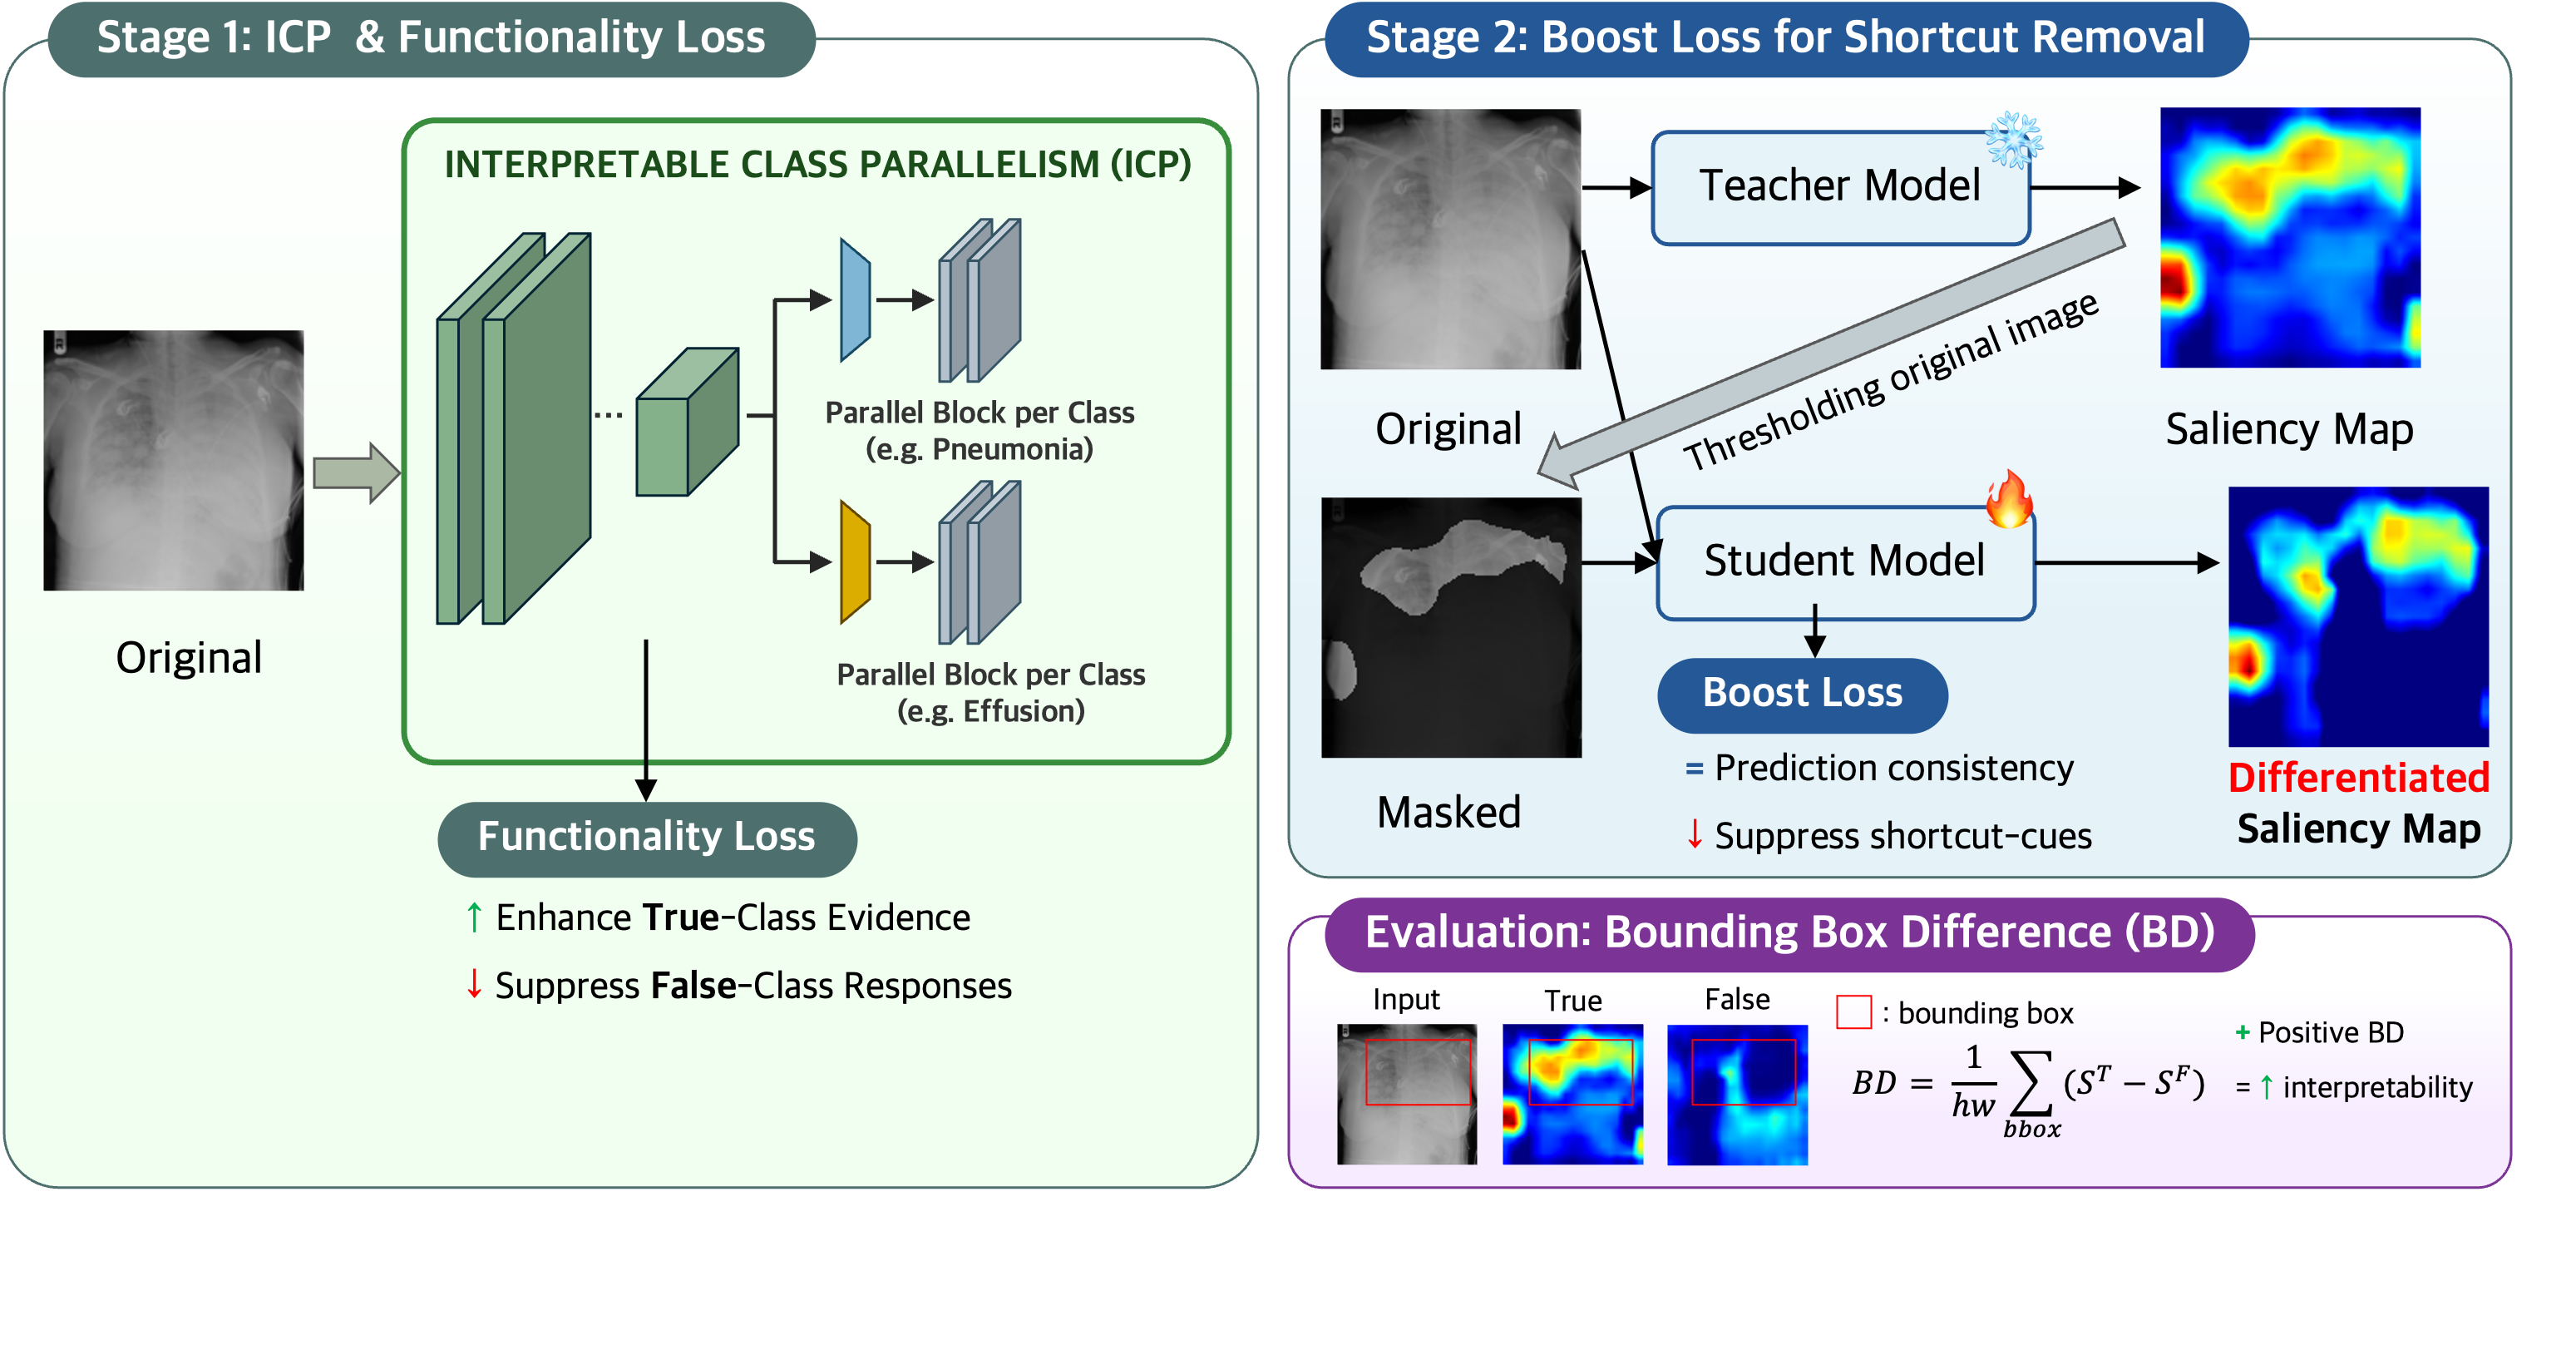
\includegraphics[width=6.0in, height=3.2in]{Figure1.png}
\caption{\textcolor{black}{Overview of the proposed saliency differentiation framework. Stage 1 replaces the shared final block with class-specific parallel blocks through Interpretable Class Parallelism (ICP), and optimizes the network with Functionality Loss so that saliency responses for true classes become stronger than those for false classes. Stage 2 uses a frozen copy of the Stage 1 model to generate true-class saliency masks, attenuates weakly activated regions in the input image, and trains a second copy with Boost Loss to encourage prediction consistency between original and masked inputs while further regularizing true- and false-class saliency responses. After training, interpretability is assessed with the proposed Bounding-box Difference (BD) metric, which quantifies whether true-class saliency is more activated than false-class saliency inside annotated diagnostic regions, together with deletion-based evaluation.}}
\label{fig:overall}
\end{center}
\end{figure*}

\section{Method}
\label{sec:Methods}

We propose a two-stage training framework \textcolor{red}{that generates distinct saliency maps for true and false classes to improve performance and interpretability simultaneously.} \textcolor{black}{The framework operationalizes a clinically motivated prior: diagnostic predictions should be supported by regions that contain visual evidence for the target findings.} \textcolor{red}{Figure \ref{fig:overall}} illustrates the complete workflow of our method.

    \subsection{\textcolor{black}{Overview of the Two-Stage Training Framework for Improving Diagnostic Reliability and Interpretability}}

\textbf{First Stage (Sections 4.2, 4.3, 4.4):} We modify the network architecture by replacing the final block with parallel class-specific blocks. This architectural change, which we call Interpretable Class Parallelism (ICP), enables the network to generate distinct feature representations for each class. We train this \textcolor{red}{network with a loss} that encourages each parallel block to focus on features relevant to its assigned class. \textcolor{red}{For this purpose, we propose Functionality Loss and Detailed-CAM (DCAM), which computes the saliency map of each block.}\\
\indent \textbf{Second Stage (Sections 4.5 and 4.6):} \textcolor{black}{We further regularize the model by introducing an additional training phase. \textcolor{red}{Starting from} the network trained in \textcolor{red}{Stage 1}, we generate saliency-guided masked inputs from a frozen copy of the Stage 1 model and train a second copy with Boost Loss. This loss encourages prediction consistency between original and masked inputs while increasing the relative activation of true-class saliency maps over false-class saliency maps.}\\
\indent \textbf{New Metric (Section 4.7):} We introduce \textcolor{red}{Bounding-box Difference (BD),} \textcolor{red}{an} evaluation metric that addresses limitations \textcolor{red}{of} existing \textcolor{red}{interpretability measures}.


\subsection{Interpretable Class Parallelism (ICP)}
\label{m1}

To improve performance and interpretability, previous studies have attempted to generate distinct saliency maps for different classes \cite{1, 4, 7}. However, this approach has a fundamental limitation: \textcolor{red}{because} all classes use the same underlying features, the resulting saliency maps often show insufficient differentiation between true and false classes.\\
\indent To address this limitation, we modify the network architecture by replacing the last network block with a set of parallel blocks, each corresponding to a specific class. Unlike DFU$\_$SPNet \cite{43}, which employs 3 blocks of parallel convolution layers with multiple kernel sizes, our method \textcolor{red}{applies a} simpler parallelization right before the fully connected layer. \textcolor{red}{This placement yields} heterogeneous saliency maps, \textcolor{red}{because} each parallel block can specialize in features relevant to its assigned class.\\
\indent The \textcolor{red}{saliency maps of true and false classes} obtained from this architecture \textcolor{red}{are defined as follows}:


\begin{equation}
    \mathcal{S}^T = \frac{1}{\sum_{c=1}^C \bm{1}(l_c=1)} \sum_{c=1}^C \bm{1} (y=l_c = 1) \cdot \mathcal{S}_c
    \label{eq5}
\end{equation}

\begin{equation}
    \mathcal{S}^F = \frac{1}{\sum_{c=1}^C \bm{1}(l_c=0)} \sum_{c=1}^C \bm{1} (l_c = 0) \cdot \mathcal{S}_c
    \label{eq6}
\end{equation}

$\mathcal{S}$ represents the saliency map, $T$ denotes the true class, and $F$ refers to the false class. $\mathcal{S}^T$ indicates the saliency map of the true classes, and $\mathcal{S}^F$ indicates the saliency map of the false classes. $C$ is the number of classes and $c$ is the index of a class.

ICP addresses this limitation by creating a dedicated processing pathway for each class. Specifically, we replace the last network block with a set of parallel blocks—one for each class in the classification task. Unlike the approach in \cite{44}, which employs parallel blocks throughout the entire network, we apply parallelization only to the final block before the fully connected layer. \textcolor{red}{This design (1) keeps feature extraction efficient in earlier layers, where general features are learned, (2) allows specialization in higher layers, where class-specific features become more important, and (3) uses fewer parameters than parallelizing the full network.}

Each parallel block can thus \textcolor{red}{learn a feature extractor optimized for its assigned class, which yields a more distinct and informative saliency map for each class.}



\subsection{Functionality Loss}
\label{m2}

To maximize the distinction between true and false class activations in our Interpretable Class Parallelism (ICP) architecture, we introduce \textcolor{red}{Functionality Loss. It} serves two purposes: (1) enhancing the activation of saliency maps for true classes, and (2) suppressing the activation of saliency maps for false classes.

\textcolor{red}{Functionality Loss compares the saliency maps generated by the parallel blocks according to their class labels. For each pixel position $(i, j)$, we compute the ratio of the false-class saliency value to the sum of the true- and false-class saliency values. We then sum this ratio over all pixel positions (Eq.~\ref{eq4}):}


\begin{equation}
    \begin{split}
        \mathcal{L}_{func}
        = \sum^{H}_{i=1}\sum^{W}_{j=1}\frac
        {\mathcal{S}^{F}_{ij}}
        {\mathcal{S}^{T}_{ij}+\mathcal{S}^{F}_{ij}}
    \end{split}
\label{eq4}
\end{equation}

\begin{equation}
    \mathcal{L}_{total} = \mathcal{L}_{BCE}(y, l) + \mathcal{L}_{func}(\mathcal{S}^T, \mathcal{S}^F)
    \label{eq11}
\end{equation}

In Eq. \ref{eq4}, $H$ and $W$ are the height and width of the input image, respectively, and $i$ and $j$ are the indices of the vertical and horizontal pixels. \textcolor{red}{Eq.~\ref{eq11} gives the overall training loss}, where $\mathcal{L}_{BCE}$ \textcolor{red}{is the binary cross-entropy loss}. In Eq. \ref{eq11}, $y$ is the final logit vector and $l$ is the ground truth label vector.

\subsection{Detailed-CAM (DCAM): Saliency Map for Functionality Loss}

To improve the Functionality Loss, we introduce Detailed-CAM (DCAM), a modified version of Grad-CAM that can be easily applied to both CNNs and Transformers. \textcolor{red}{This modification is motivated by the observation that Grad-CAM often yields weak activation in false-class saliency maps. When these saliency values approach zero, false classes contribute almost nothing to the Functionality Loss. Weak false-class activation might seem desirable, but Functionality Loss needs non-trivial values from both true and false classes to minimize their ratio effectively. We therefore need a saliency map that represents these values so that the loss can suppress them.}

\textcolor{red}{We modify Grad-CAM to map negative values to positive ones through the sigmoid function, which increases the Functionality Loss. Because the loss sums these sigmoid-mapped values, minimizing it further suppresses the originally negative values. To implement this, we refine the class-discriminative localization map of Grad-CAM as in Eq.~\ref{eq2}:} 


    \begin{equation}
        \underbrace{
            \frac{1}{Z}\sum_{i}\sum_{j}\frac{\partial y_c}{\partial A^{k}_{ij}}
        }_{\alpha_{k,\text{Grad-CAM}}}
        \rightarrow
        \underbrace{
            \sigma\bigg(\frac{1}{Z}\sum_{i}\sum_{j}\frac{\partial y_c}{\partial A^{k}_{ij}}\bigg)
        }_{\alpha_{k,\text{DCAM}}}
    \label{eq2}
    \end{equation}

To implement these modifications, we first adjust the gradient weights. In Eq. \ref{eq2}, we scale the global average pooling results to the range [0, 1] using the sigmoid function, $\sigma$, to over-represent small values and aid in their suppression. Here, $A$ represents the activation map, $\sigma$ is the sigmoid function, \textcolor{red}{$y_c$} is the score of the $c^{th}$ category\textcolor{red}{, and $k$ indexes the activation maps.}
    
    \begin{equation}
        \underbrace{
            \text{ReLU}\bigg(\sum_{k}\alpha_{k,\text{CAM}} * A^{k}\bigg)
        }_{S_\text{Grad-CAM}}
        \rightarrow
        \underbrace{
            \sigma\bigg(\sum_{k}\alpha_{k,\text{DCAM}} * A^{k}\bigg)
        }_{S_\text{DCAM}}
    \label{eq3}
    \end{equation}

Furthermore, we replace ReLU with the sigmoid function when calculating the final saliency map $S$ (a weighted combination of forward activation maps). \textcolor{red}{This replacement keeps the information in negative values and maps them to positive values, so that the loss can suppress them further.}

\textcolor{red}{Figure \ref{fig:CAM} compares DCAM with standard Grad-CAM and partial modifications. Applying Grad-CAM to ICP resulted in weak activation in false-class saliency maps and, in some cases, poor activation in true-class saliency maps. This is problematic because the numerator of Functionality Loss is the false-class saliency, so the loss approaches zero. The modifications in Eq.~\ref{eq2} and Eq.~\ref{eq3} produce positive activation in false-class saliency maps. As a result, false-class pixels with larger magnitudes, whether originally positive or negative, increase the Functionality Loss. Each modification alone improves false-class activation, but it either differentiates true and false classes insufficiently (Eq.~\ref{eq2} alone) or activates false classes excessively (Eq.~\ref{eq3} alone). DCAM combines both and balances the two effects: false classes receive meaningful activation values while remaining sufficiently differentiated from true classes. With DCAM, the model can use Functionality Loss more effectively to improve classification performance and interpretability simultaneously.}


\subsection{Masking Strategy Through Dual-Network Thresholding}
\label{m3}

\textcolor{black}{To reduce the model's sensitivity to weakly attributed peripheral regions, we propose a saliency-guided input masking strategy. In medical imaging, models may exploit artifacts, background patterns, or other dataset-specific cues that are not directly related to the visual evidence of disease. Rather than claiming to remove all such shortcuts, our framework regularizes the model so that its predictions are preserved when low-saliency regions are attenuated.}
\textcolor{black}{Specifically, we use the \textcolor{red}{activation} of the true-class saliency map as a guiding signal. In \textcolor{red}{Stage 1}, the model is trained with ICP and Functionality Loss until convergence. In \textcolor{red}{Stage 2}, we duplicate the trained Stage 1 model: one copy is frozen and used to generate saliency masks, while the other copy is trainable and optimized with Boost Loss.}

\textcolor{red}{We prepare masked images as follows. First, we feed input images into the frozen model to generate saliency maps. We then threshold these saliency maps to obtain masks:}

\begin{equation}
    M_{ij} = \begin{cases} 
1 & \text{if } \mathcal{S}_{ij}^T \geq \tau \\
\psi & \text{otherwise}
\label{eq:mask}
\end{cases}
\end{equation}

$M$ is the mask\textcolor{red}{, and $i$ and $j$ are the horizontal and vertical pixel indices.} $\tau$ is \textcolor{red}{a threshold hyperparameter determined empirically, and $\psi$ is a masking hyperparameter that decreases the intensity of a pixel. We then apply this mask to obtain the masked input image:}

\begin{equation}
    x'_{ij} = x_{ij} * M_{ij}
    \label{eq7}
\end{equation}

\textcolor{red}{where} $x$ is \textcolor{red}{the} original input image and $x'$ is the masked image.

\textcolor{black}{Next, \textcolor{red}{we feed} the masked image $x'$ and the original image $x$ \textcolor{red}{into} the trainable model \textcolor{red}{and} obtain two logit vectors and two sets of true- and false-class saliency maps, $\mathcal{S}^{MT}$, $\mathcal{S}^{OT}$, $\mathcal{S}^{OF}$, and $\mathcal{S}^{MF}$. $O$ indicates the original input and $M$ indicates the masked input. Therefore, $\mathcal{S}^{MT}$ and $\mathcal{S}^{OT}$ are the true-class saliency maps from masked and original images, respectively, while $\mathcal{S}^{MF}$ and $\mathcal{S}^{OF}$ are the false-class saliency maps from masked and original images, respectively. $W$ and $H$ represent the width and height of the saliency maps.}

\subsection{Boost \textcolor{red}{Loss}}
\label{m4}

\textcolor{black}{Medical image classification models may rely on peripheral or dataset-specific features rather than diagnostically relevant regions \cite{45, 46}. For example, models can learn correlations with hospital markers, text annotations, background patterns, or other non-pathological cues in chest X-rays \cite{47,15}. To address this limitation, we introduce Boost Loss, which regularizes the model using saliency-guided masked inputs and encourages prediction stability when weakly attributed regions are attenuated.}

\textcolor{black}{\textcolor{red}{Boost Loss is computed from the logits and saliency maps of both the original and the saliency-masked inputs.} It consists of two components. The first component (Eq. \ref{eq9}) uses \textcolor{red}{the pre-sigmoid logits} $z$ and minimizes the distance between logits from the original and masked inputs.}


\begin{equation}
    \frac{1}{C} \sum_{i=1}^C |z^O_i - z^M_i| 
    \label{eq9}
\end{equation}

\textcolor{black}{Here, $i$ is the class index and $C$ is the total number of classes. The masked-input logit $z^M$ is derived from $x'$, where regions with weak true-class saliency are attenuated. By reducing the distance between $z^O$ and $z^M$, this term encourages the trainable model to make consistent decisions whether the weakly attributed regions are visible or suppressed.}

\textcolor{black}{This component functions as a consistency regularizer. Because the masked input $x'$ is generated from the frozen Stage 1 model's saliency map, it preserves regions that the model identifies as evidence for true classes while reducing the intensity of less activated regions. Therefore, minimizing the distance between $z^O$ and $z^M$ encourages the trainable model to rely on evidence that remains available after saliency-guided masking.}

\textcolor{black}{The second component (Eq. \ref{eq10}) compares true- and false-class saliency maps obtained from original and masked inputs. The first ratio encourages true-class saliency in the original input to remain at least as strong as that in the masked input. The second ratio discourages false-class saliency in the original input from exceeding false-class saliency under masking. Together, these terms regularize the relative saliency behavior of true and false classes under saliency-guided perturbation.}


\begin{equation}
    \textcolor{black}{\frac{\sum_{i=1}^W \sum_{j=1}^H \mathcal{S}_{ij}^{MT}}{\sum_{i=1}^W\sum_{j=1}^H \mathcal{S}_{ij}^{OT}} + \frac{\sum_{i=1}^W \sum_{j=1}^H \mathcal{S}_{ij}^{OF}}{\sum_{i=1}^W \sum_{j=1}^H \mathcal{S}_{ij}^{MF}}}
    \label{eq10}
\end{equation}

\textcolor{red}{The full Boost Loss is:}

\begin{equation}
    \textcolor{black}{\mathcal{L}_{boost} = \gamma * \frac{1}{C} \sum_{i=1}^C |z^O_i - z^M_i| + \beta * \left(\frac{\sum_{i=1}^W \sum_{j=1}^H \mathcal{S}_{ij}^{MT}}{\sum_{i=1}^W\sum_{j=1}^H \mathcal{S}_{ij}^{OT}} + \frac{\sum_{i=1}^W \sum_{j=1}^H \mathcal{S}_{ij}^{OF}}{\sum_{i=1}^W \sum_{j=1}^H \mathcal{S}_{ij}^{MF}}\right)}
\end{equation}

\textcolor{red}{The} hyperparameters $\gamma$ and $\beta$ \textcolor{red}{control the contributions of the first and second terms. In our experiments, setting them independently worked better than coupling them.}

\textcolor{black}{As a result, Boost Loss encourages stable predictions under saliency-guided masking while further differentiating true- and false-class saliency maps. This loss is clinically motivated because diagnostic evidence in chest X-ray images should be supported by image regions containing relevant anatomical or pathological patterns rather than by weakly attributed peripheral information.}

Finally, we train the trainable model with the \textcolor{red}{loss} in \textcolor{red}{Eq.~\ref{eq8}}: 

\begin{equation}
    \textcolor{black}{\mathcal{L}_{total} = \mathcal{L}_{BCE}(y, l) + \mathcal{L}_{boost}(z^O, z^M, \mathcal{S}^{OT}, \mathcal{S}^{OF}, \mathcal{S}^{MT}, \mathcal{S}^{MF})}
    \label{eq8}
\end{equation}

\subsection{Bounding-box Difference (BD)}
\label{m5}

While several metrics exist for evaluating classification performance, quantitative measures for assessing interpretability in medical imaging remain limited. \textcolor{red}{The deletion score \cite{84} measures classification performance after the highly activated regions of saliency maps are erased from the original X-ray images. It cannot, however, measure whether the model bases its decisions on the critical regions that contain evidence of disease. In addition, saliency maps are currently evaluated through qualitative assessment by experts, which is subjective and makes different results difficult to compare.} To mitigate this limitation, we propose the \textcolor{red}{Bounding-box} Difference (BD) metric, \textcolor{red}{which quantifies how strongly a model focuses on} diagnostically relevant regions.

This metric directly corresponds to the interpretability conditions established in Section 3.2, particularly Condition 2, which states that saliency maps for true classes should show stronger activation in critical regions compared to those of false classes.

\textcolor{red}{BD measures how much more strongly the true-class saliency map is activated in the critical region, often given as a bounding box, than the false-class saliency map. It provides} a quantitative baseline for evaluating model interpretability. Specifically, we obtain saliency maps for \textcolor{red}{the} true and false classes \textcolor{red}{with} a chosen method (e.g., Grad-CAM or DCAM) \textcolor{red}{and define a bounding box around the critical region. The BD score subtracts the sum of false-class saliency values inside the bounding box from that of true-class saliency values and normalizes it by the box area:}


\begin{equation}
    \frac{\sum_{i=m}^{m+h}\sum_{j=n}^{n+w} (\mathcal{S}_{ij}^T - \mathcal{S}_{ij}^{F})}{h * w} * 100
\end{equation}

Here, $i$ and $j$ denote the indices of the pixels in the image, while $m$ and $n$ represent the starting indices of the bounding box, and $h$ and $w$ are the height and width of the bounding box, respectively. $\mathcal{S}$ refers to the saliency map. \textcolor{red}{We multiply the score by 100 to adjust its scale. Figure~\ref{fig:overall} illustrates this procedure.}

\textcolor{red}{The resulting} BD score quantifies the relative activation levels between true and false classes within critical regions. Positive BD values represent stronger activation for true classes compared to false classes within the critical region, suggesting good interpretability. BD values near zero \textcolor{red}{indicate} similar activation levels for both true and false classes, suggesting poor differentiation and potentially problematic interpretability. Negative BD values \textcolor{red}{indicate} stronger activation for false classes within the critical region, suggesting severely flawed model attention.

This metric provides a straightforward way to quantitatively evaluate the relative activation levels of true and false class saliency maps, offering insights into the interpretability of the model. \textcolor{red}{With this metric, we can compare the interpretability of different models and methods systematically. It can thus help identify whether a model attends to appropriate features.} However, because it depends on \textcolor{red}{an} accurate definition of critical regions, it may not fully capture complex attention patterns that extend beyond the defined regions. Despite these limitations, the BD metric serves as a valuable quantitative baseline for evaluating model interpretability in medical imaging tasks, complementing traditional performance metrics and qualitative assessments.


\subsection{\textcolor{black}{Optimization Perspective}}

\textcolor{black}{The proposed losses are designed to increase the relative saliency activation of true classes over false classes. We provide an optimization-level interpretation in Appendix \ref{Appendix:D}, showing how reducing overlap between true- and false-class saliency maps is consistent with the objective optimized by Functionality Loss.}

\begin{figure*}
\begin{center}
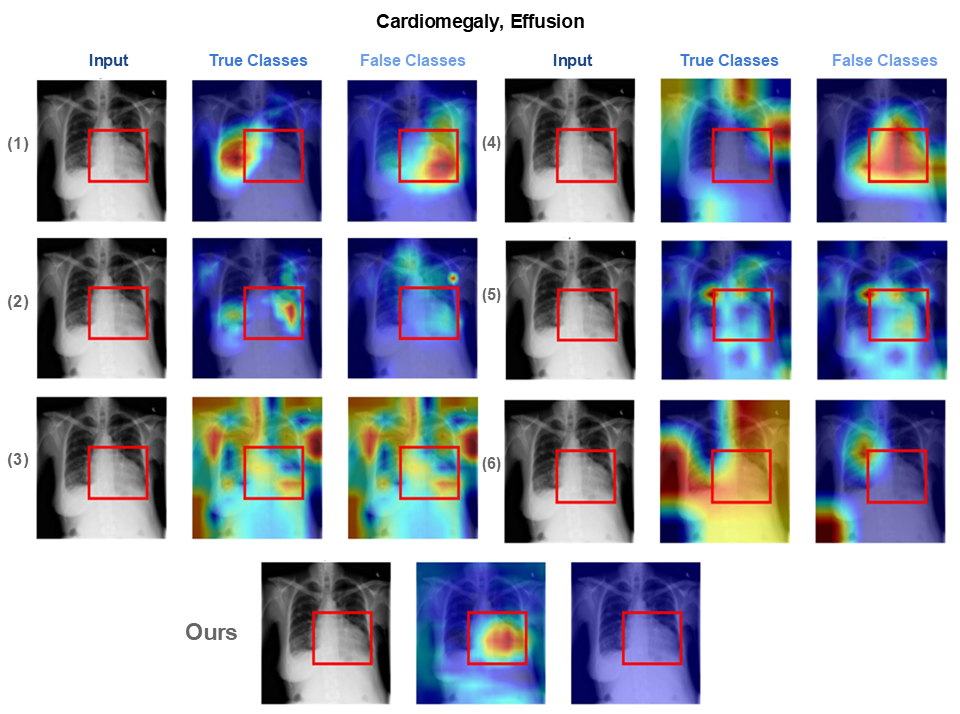
\includegraphics[width=5in, height=3.7in]{Figure4.png}
\caption{\textcolor{red}{Comparison of Grad-CAM saliency maps across model architectures:} (1) ResNet18\textcolor{red}{,} (2) ResNet18 with $\mathcal{L}_{AS}$\textcolor{red}{,} (3) ViT\textcolor{red}{,} (4) \textcolor{red}{ConvNeXt-Base}, (5) DenseNet121\textcolor{red}{, and} (6) \textcolor{red}{EfficientNetB7}. \textcolor{red}{The last row shows our method, ICP-XL with Stage 2.}}
\label{fig:comparison}
\end{center}
\end{figure*}

\begin{figure*}
\begin{center}    
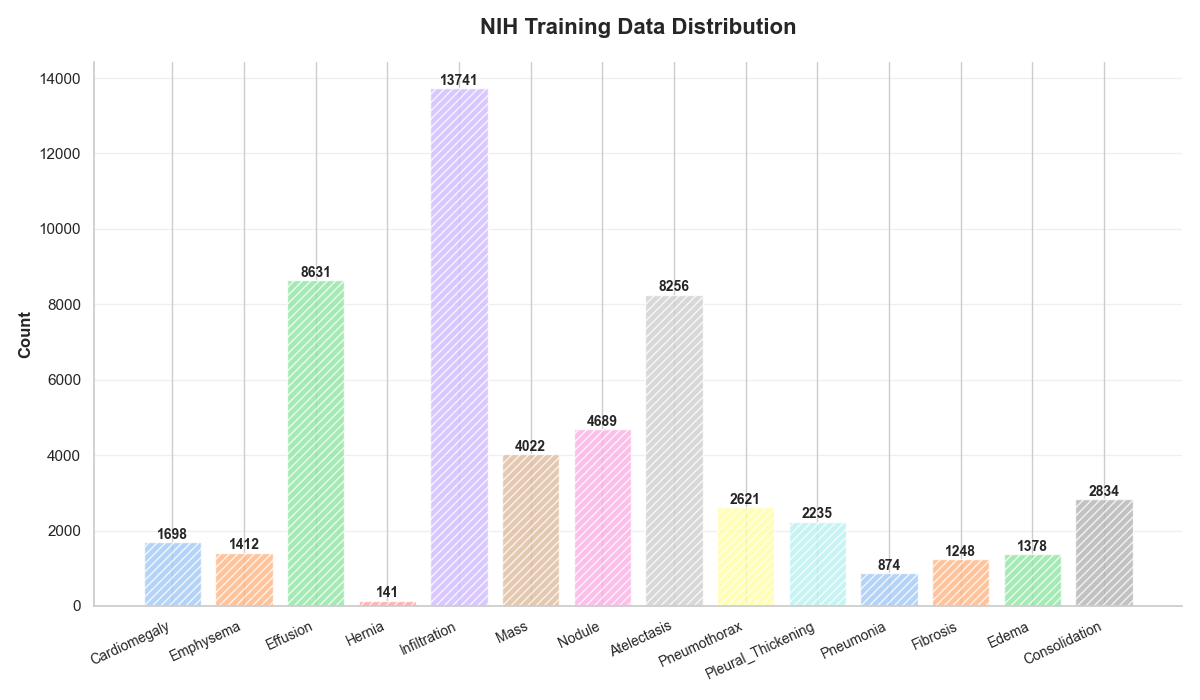
\includegraphics[width=3.0in]{figs/NIH_train_distribution.png}
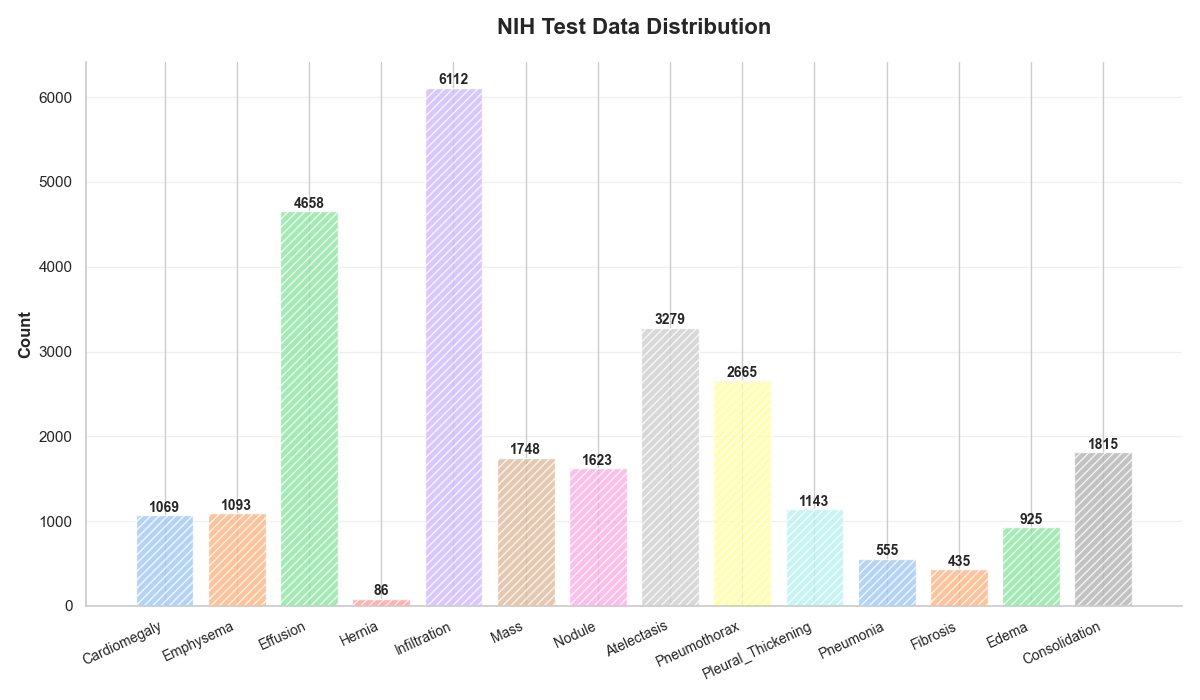
\includegraphics[width=3.0in]{figs/NIH_test_distribution.png}
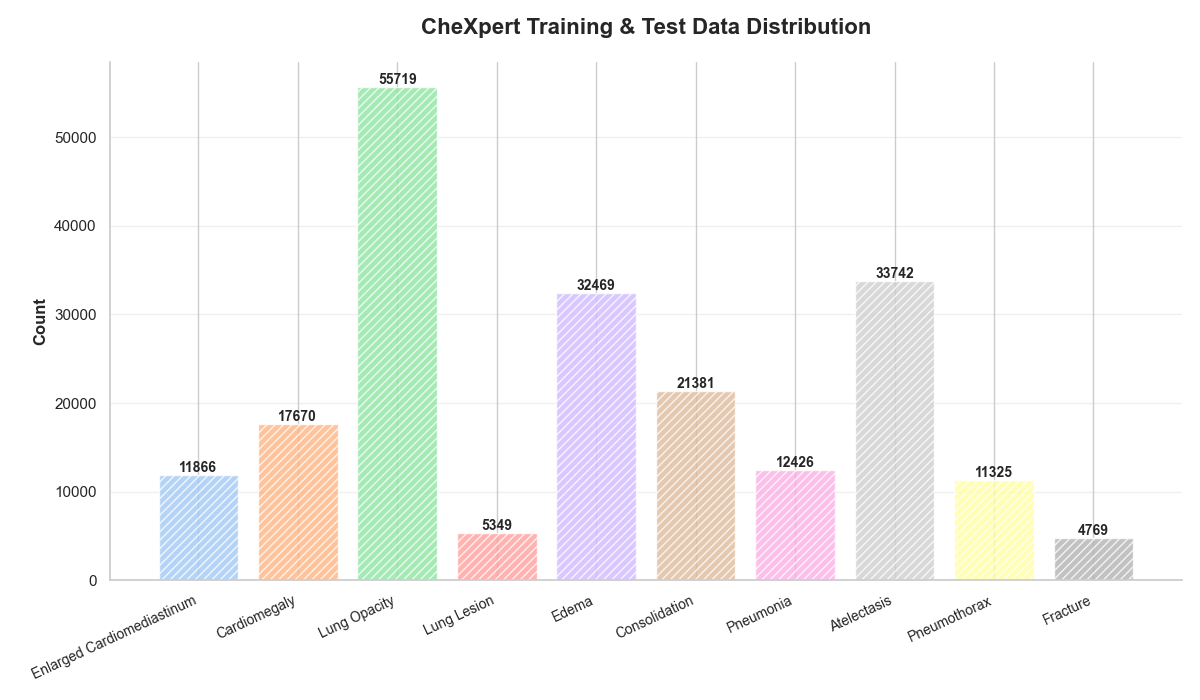
\includegraphics[width=3.0in]{figs/CheXpert_train_test_distribution.png}
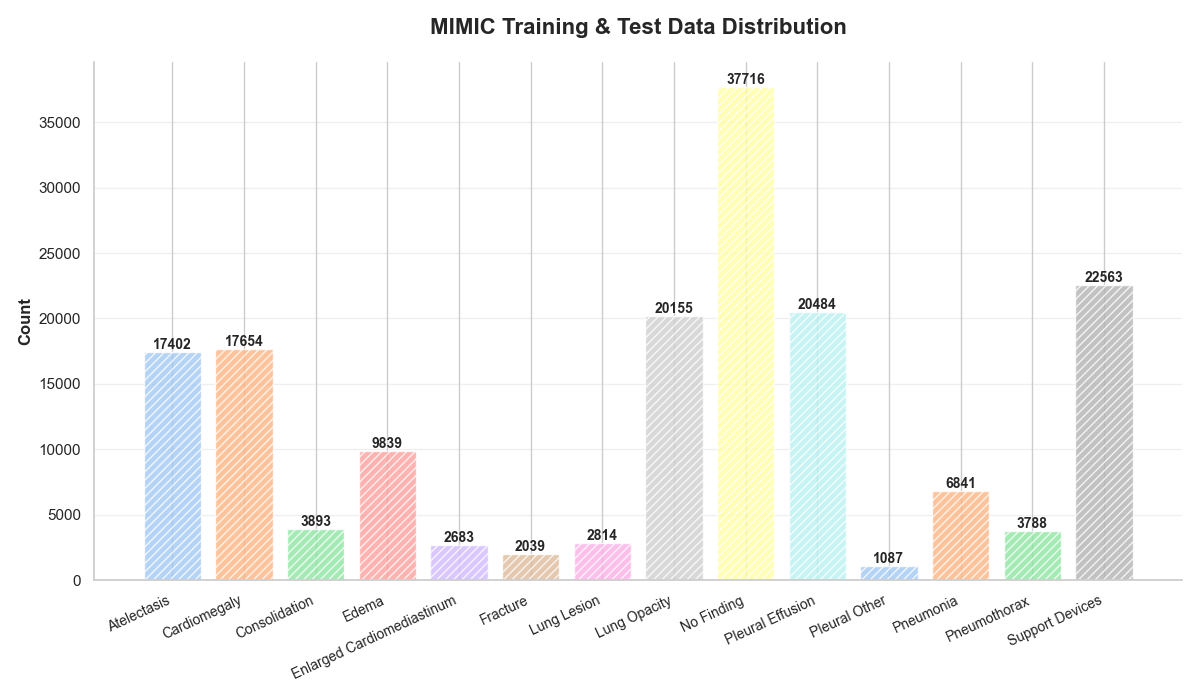
\includegraphics[width=3.0in]{figs/MIMIC_train_test_distribution.png}
\end{center}
\caption{\textcolor{red}{Class distributions of all datasets used in this study. NIH CXR 14 has designated training and test sets, so we show them separately. For CheXpert and MIMIC-CXR, we randomly sampled and split the data, so we show the merged training and test distribution.}}
\label{fig:dist}
\end{figure*}

\section{Experiment}
\label{sec:results}

We conducted experiments on \textcolor{red}{several} large-scale \textcolor{red}{chest} X-ray datasets. \textcolor{black}{In Stage 1, we compare the proposed ICP-based models with baseline architectures, including DenseNet121, EfficientNetB7, ConvNeXtBase, Vision Transformer (ViT), and ResNet18-based training objectives. To evaluate Stage 2, we compare models trained with and without the proposed Boost Loss after Stage 1 initialization.} \textcolor{red}{Appendix \ref{Appendix2} describes the datasets and experimental details.}

\subsection{Datasets}
We \textcolor{red}{used three} large-scale chest X-ray \textcolor{red}{datasets}\textcolor{red}{: NIH ChestX-ray 14 \cite{82}, CheXpert \cite{48}, and MIMIC-CXR.} \textcolor{red}{First}, NIH ChestX-ray 14 (NIH CXR 14) has 14 disease labels ('Cardiomegaly', 'Emphysema', 'Effusion', 'Hernia', 'Infiltration', 'Mass', 'Nodule', 'Atelectasis', 'Pneumothorax', 'Pleural Thickening', 'Pneumonia', 'Fibrosis', 'Edema', 'Consolidation', 'No Finding')\textcolor{red}{, and we used all of them. It contains only frontal views, with 86,336 training and 25,596 test samples. Because its labels were extracted from clinical reports with natural language processing, some labels are erroneous. The dataset provides multi-label class labels and bounding-box (B-Box) labels for 984 images. Each B-Box label contains the starting coordinates, width, and height of the box. The bounding boxes were manually annotated by board-certified radiologists on sampled images, guided by disease keywords extracted from the radiological reports in the institution's PACS system. For preprocessing, we applied normalization. For Stage 1, we used the original training and test sets. For Stage 2, we additionally sampled 10,000 validation images from the training set, because Stage 2 is intended to calibrate the decision boundaries with the knowledge that the model acquired during Stage 1.}

Second, CheXpert \textcolor{red}{contains 224,316 chest radiographs of 65,240 patients, with frontal and lateral views, and} 14 disease labels ('Atelectasis', 'Cardiomegaly', 'Consolidation', 'Edema', 'Effusion', 'Pneumonia', 'Pneumothorax', 'Enlarged Cardiomediastinum', 'Fracture', 'Pleural Other', 'Lung Opacity', 'Lung Lesion', 'Support Devices', 'No Finding'). \textcolor{red}{Following previous work, we excluded ambiguous labels (``No Finding,'' ``Support Devices,'' ``Pleural Effusion,'' and ``Pleural Other''). For Stage 1, we used 86,336 training and 22,366 test images without a validation set. For Stage 2, we randomly sampled 10,000 validation images from the training set.}

Lastly, MIMIC-CXR \textcolor{red}{consists of 377,110 chest X-ray images of 65,379 patients, from which we sampled 100,000 images. It contains} 14 disease labels ('Atelectasis', 'Cardiomegaly', 'Consolidation', 'Edema', 'Enlarged Cardiomediastinum', 'Fracture', 'Lung Lesion', 'Lung Opacity', 'No Finding', 'Pleural Effusion', 'Pleural Other', 'Pneumonia', 'Pneumothorax', 'Support Devices') \textcolor{red}{and, like CheXpert, has no bounding-box labels. We used 72,000, 8,000, and 20,000 images for training, validation, and testing, respectively.}

\textcolor{red}{Figure \ref{fig:dist} shows the class distributions of NIH CXR 14, CheXpert, and MIMIC-CXR.}

\subsection{Experiments of Stage 1}

\textcolor{red}{In Stage 1, we train each model until convergence, and in our experiments 20 epochs were sufficient. Tables \ref{tab:1} and \ref{tab:2} show the Stage 1 results on NIH CXR 14 and CheXpert. We compare our methods with the Attention Separation Loss ($\mathcal{L}_{AS}$) of Improving Classification with Attention Separation and Consistency (ICASC) \cite{7}, which increases the difference between the saliency maps of different classes in multi-class classification of natural images. We also evaluate the combination of $\mathcal{L}_{AS}$ and $\mathcal{L}_{func}$. We do not report the attention consistency loss of ICASC, because its fixed hyperparameters prevented it from producing meaningful results. BD denotes Bounding-box Difference, and DT and DF denote the deletion scores of true and false classes. \# Params is the number of model parameters. ICP-T, ICP-M, ICP-L, and ICP-XL are ICP with 1, 128, 256, and 512 channels, respectively. We used three random seeds for all experiments. Appendix \ref{Appendix2} explains the metrics in detail.}



\begin{table*}
    \centering
    {\resizebox{\textwidth}{!}{
    \begin{tabular}{c|cc|c|cccc|c}
        \toprule
        \multicolumn{9}{c}{\textbf{NIH CXR 14}}\\
        \midrule
        \textbf{Method} & $\mathbf{\mathcal{L}_{AS}}$ & $\mathbf{\mathcal{L}_{func}}$& \textbf{\textcolor{magenta}{AUC $\uparrow$}} & \textbf{\textcolor{cyan}{BD $\uparrow$}} & \textbf{\textcolor{cyan}{DT $\uparrow$}}& \textbf{\textcolor{cyan}{DF $\downarrow$}}& \textbf{\textcolor{cyan}{DT - DF $\uparrow$}} & \textbf{\# Params}\\
        \midrule
        \rowcolor{Gray}
        DenseNet121 & X & X & 70.61 $(\pm0.97)$ & 1.17 $(\pm0.85)$ & 0.92 $(\pm0.45)$ & 2.80 $(\pm1.41)$ & -1.75 $(\pm1.75)$ & 7M\\
        \rowcolor{Gray}
        EfficientNetB7 & X & X & 68.64 $(\pm0.30)$ & 3.04 $(\pm0.66)$ & \textbf{13.55} $\bm{(\pm2.49)}$ & 4.31 $(\pm0.20)$ & \textbf{9.31} $\bm{(\pm2.62)}$ & 63M\\
        \rowcolor{Gray}
        ConvNeXtBase & X & X & 59.76 $(\pm0.33)$ & -3.34 $(\pm3.34)$ & 6.38 $(\pm0.41)$ & 0.70 $(\pm0.25)$ & 5.54 $(\pm0.55)$ & 87M\\
        \rowcolor{Gray}
        ViT & X & X & 66.54 $(\pm1.05)$ & 0.00 $(\pm0.00)$ & 13.44 $(\pm0.78)$ & 13.44 $(\pm0.78)$ & 0.00 $(\pm0.00)$ &  85M\\
        \rowcolor{Gray}
        ResNet18 & X & X & 66.59 $(\pm0.16)$ & -24.64 $(\pm0.17)$ & 8.64 $(\pm0.97)$ & 6.61 $(\pm0.67)$ & 2.06 $(\pm1.61)$ & 11M\\
        \rowcolor{Gray}
        ResNet18 & O & X & 67.91 $(\pm0.23)$ & -19.10 $(\pm 2.10)$& 5.74$(\pm0.05)$& 1.79 $(\pm1.71)$& 3.95 $(\pm1.77)$ & 11M\\
        \midrule
        ResNet18 & X & O & 66.97 $(\pm0.25)$ & 2.03 $(\pm 0.45)$& 8.25 $(\pm0.14)$& 6.63 $(\pm0.76)$& 1.62 $(\pm0.62)$ & 11M\\
        ResNet18 & O & O & 66.86 $(\pm0.60)$ & 3.20 $(\pm0.61)$&3.59 $(\pm0.56)$& 0.11 $(\pm0.02)$& 3.48 $(\pm0.54)$ & 11M\\
        \midrule
        ICP-T & X & X & 68.88 $(\pm0.21)$& 2.51 $(\pm2.24)$& 0.26 $(\pm0.23)$& 0.01 $(\pm0.01)$& 0.26 $(\pm0.23)$ & 11M\\
        ICP-T & O & X & 69.52 $(\pm 0.69)$ & 3.25 $(\pm2.82)$& 0.18 $(\pm0.06)$& 0.00 $(\pm0.02)$& 0.19 $(\pm0.05)$ & 11M\\
        ICP-T & X & O & 69.55 $(\pm0.86)$ & 8.69 $(\pm6.79)$ & 1.57 $(\pm1.24)$& \textbf{0.00} $\bm{(\pm0.00)}$& 1.56 $(\pm1.24)$ & 11M\\
        ICP-T & O & O & 65.69 $(\pm1.99)$& 16.78 $(\pm1.83)$& 2.30 $(\pm0.06)$& 0.07 $(\pm0.07)$& 2.26 $(\pm0.04)$ & 11M\\
        \midrule
        ICP-M & X & X & 71.86 $(\pm0.99)$ & 8.92 $(\pm6.26)$ & 2.69 $(\pm1.17)$& \textbf{0.00} $\bm{(\pm0.00)}$ & 2.69 $(\pm1.17)$& 21M\\
        ICP-M & O & X & 72.56 $(\pm0.83)$& 1.87 $(\pm0.88)$& 0.79 $(\pm0.51)$& \textbf{0.00} $\bm{(\pm0.00)}$ & 0.79 $(\pm0.51)$ & 21M\\
        ICP-M & X & O & 74.38 $(\pm0.88)$ & 16.59 $(\pm1.52)$ & 5.75 $(\pm0.45)$& \textbf{0.00} $\bm{(\pm0.00)}$ & 5.75 $(\pm0.45)$ & 21M\\
        ICP-M & O & O & 72.69$(\pm1.27)$& 3.17 $(\pm1.47)$& 0.33 $(\pm0.32)$& \textbf{0.00} $\bm{(\pm0.00)}$ & 0.33 $(\pm0.32)$ & 21M\\
        \midrule
        ICP-L & X & X & 71.03 $(\pm1.02)$ & 3.91 $(\pm3.58)$ & 1.34 $(\pm1.03)$& \textbf{0.00} $\bm{(\pm0.00)}$ & 1.34 $(\pm1.03)$ & 45M\\
        ICP-L & O & X & 73.64 $(\pm0.72)$& 0.53 $(\pm0.14)$& 0.23 $(\pm0.13)$& \textbf{0.00} $\bm{(\pm0.00)}$ & 0.23 $(\pm0.13)$ & 45M\\
        \rowcolor{LemonChiffon1}
        ICP-L & X & O & 74.38 $(\pm0.16)$ & 16.10 $(\pm1.22)$ & 5.46  $(\pm0.70)$& 0.03 $(\pm0.02)$& 5.43 $(\pm0.72)$ & 45M\\
        ICP-L & O & O & 73.66 $(\pm 0.25)$& 2.66 $(\pm1.84)$& 0.25 $(\pm0.13)$& \textbf{0.00} $\bm{(\pm0.00)}$ & 0.25 $(\pm0.13)$ & 45M\\
        \midrule
        ICP-XL & X & X & 72.89 $(\pm1.03)$& 1.87 $(\pm1.44)$ & 1.80 $(\pm1.13)$& \textbf{0.00} $\bm{(\pm0.00)}$ & 1.80 $(\pm1.13)$ & 128M\\
        ICP-XL & O & X & 73.91 $(\pm0.36)$& 1.04 $(\pm0.54)$ & 0.14 $(\pm0.05)$& \textbf{0.00} $\bm{(\pm0.00)}$ & 0.14 $(\pm0.05)$ & 128M\\
        ICP-XL & X & O & \textbf{74.64 $\bm{(\pm0.76)}$} & \textbf{17.88 $\bm{(\pm1.69)}$} & 6.84 $(\pm0.39)$& 0.02 $(\pm0.02)$ & 6.83 $\bm(\pm0.37)$ & 128M\\
        ICP-XL & O & O & 73.78 $(\pm0.62)$& 2.69 $(\pm0.73)$& 0.44 $(\pm0.33)$& \textbf{0.00} $\bm{(\pm0.00)}$ & 0.44 $(\pm0.33)$ & 128M\\
        \bottomrule
    \end{tabular}
    }}
    \caption{Stage 1 results on NIH CXR 14. \textcolor{red}{Gray rows are baselines without our methods, and white rows are variants of our methods. The pink column reports performance, and the blue columns report interpretability.}}
    \label{tab:1}
\end{table*}

\subsubsection{NIH CXR 14}

Table \ref{tab:1} shows the results on NIH CXR 14. \textcolor{red}{With ICP, the deletion score of false classes (DF) becomes almost zero, which indicates that ICP effectively separates true and false classes. ICP with Functionality Loss improves both performance and interpretability, which is regarded as challenging. ICP with 512 channels (ICP-XL) and Functionality Loss achieves the highest results, and ICP-M with Functionality Loss achieves the second-best performance and interpretability. Because the gap between the two is small, ICP-M with Functionality Loss is a cost-effective choice given its fewer parameters.}

\begin{table*}
    \centering
    \resizebox{\textwidth}{!}{\begin{tabular}{c|cc|c|ccc|c}
        \toprule
        \multicolumn{8}{c}{\textbf{CheXpert}}\\
        \midrule
        \textbf{Method} & $\mathbf{\mathcal{L}_{AS}}$ & $\mathbf{\mathcal{L}_{func}}$ & \textbf{\textcolor{magenta}{AUC $\uparrow$}} & \textbf{\textcolor{cyan}{DT $\uparrow$}}& \textbf{\textcolor{cyan}{DF $\downarrow$}}& \textbf{\textcolor{cyan}{DT - DF $\uparrow$}} & \textbf{\# Params}\\
        \midrule
        \rowcolor{Gray}
        DenseNet121 & X & X & 66.43 $(\pm0.63)$ & 2.67 $(\pm1.11)$& 1.07 $(\pm0.22)$& 1.73 ($\pm 1.21$) & 7M\\
        \rowcolor{Gray}
        EfficientNetB7 & X & X & 66.79 $(\pm0.09)$ & 6.99 $(\pm0.49)$ & 1.15 $(\pm0.19)$& 5.78 $(\pm0.35)$& 63M\\
        \rowcolor{Gray}
        ConvNeXtBase & X & X & 60.93 $(\pm1.03)$ & 6.51 $(\pm5.26)$ & 2.38 $(\pm1.66)$ & 4.04 $(\pm3.68)$ & 87M\\
        \rowcolor{Gray}
        ViT & X & X & 64.18 $(\pm0.09)$ & 10.96 $(\pm1.22)$ & 10.96 $(\pm1.22)$ & 0.00 $(\pm0.00)$ & 85M\\
        \rowcolor{Gray}
        ResNet18 & X & X & 64.01 $(\pm0.15)$ & 8.72 $(\pm0.28)$ & -1.01 $(\pm1.42)$ & 11.28 $(\pm0.57)$ & 11M\\
        \rowcolor{Gray}
        ResNet18 & O & X & 64.69 $(\pm1.42)$ & 6.87 $(\pm0.86)$ & \textbf{-2.55} $\bm{(\pm0.85)}$ & 9.62 $(\pm1.51)$ & 11M\\
        \midrule
        ResNet18 & X & O & 63.71 $(\pm0.28)$ & 8.93 $(\pm0.69)$ & -0.02 $(\pm0.10)$ & 11.09 $(\pm0.59)$ & 11M\\
        ResNet18 & O & O & 63.55 $(\pm0.45)$ & 5.60 $(\pm0.04)$ & -1.32 $(\pm0.12)$ & 6.94 $(\pm0.15)$ & 11M \\
        \midrule
        ICP-T & X & X & 65.13 $(\pm0.31)$& 5.08 $(\pm3.09)$& -0.19 $(\pm0.16)$& 5.29 $(\pm3.24)$ & 11M\\
        ICP-T & O & X & 65.13 $(\pm0.54)$& 6.40 $(\pm3.88)$& -0.47 $(\pm0.42)$& 6.88 $(\pm4.30)$ & 11M\\
        ICP-T & X & O & 65.10 $(\pm0.84)$& 5.84 $(\pm3.89)$& -0.43 $(\pm0.41)$& 6.28 $(\pm4.31)$ & 11M\\
        ICP-T & O & O & 65.23 $(\pm0.92)$& 6.76 $(\pm3.63)$& -0.38 $(\pm0.29)$& 7.15 $(\pm3.91)$ & 11M\\
        \midrule
        ICP-M & X & X & 68.62 $(\pm0.64)$& 11.96 $(\pm0.36)$& -0.11 $(\pm0.14)$& 12.07 $(\pm0.26)$ & 18M\\
        ICP-M & O & X & 68.40 $(\pm0.43)$& 11.86 $(\pm0.08)$& -0.19 $(\pm0.20)$& 12.23 $(\pm0.85)$ & 18M\\
        \rowcolor{LemonChiffon1}
        ICP-M & X & O & 69.09 $(\pm0.71)$& \textbf{12.22} $\bm{(\pm1.32)}$& -0.11$(\pm0.11)$& \textbf{12.34 }$(\bm{\pm1.21)}$ & 18M\\
        ICP-M & O & O & 68.13 $ (\pm0.25)$& 11.63 $(\pm1.45)$& 0.19 $(\pm0.31)$& 11.43 $(\pm1.24)$ & 18M\\
        \midrule
        ICP-L & X & X & 65.98 $(\pm0.96)$& 3.17 $(\pm2.41)$& -0.14 $(\pm0.02)$& 3.32 $(\pm2.44)$ & 35M\\
        ICP-L & O & X & 66.48 $(\pm 0.20)$& 1.19 $(\pm0.51)$ & -0.06 $(\pm0.05)$ & 1.27 $(\pm0.52)$ & 35M\\
        ICP-L & X & O & 67.65 $(\pm1.32)$ & 10.66 $(\pm1.05)$ & -0.42 $(\pm0.36)$ & 11.09 $(\pm1.42)$ & 35M\\
        ICP-L & O & O & 69.74 $(\pm0.95)$& 2.82 $(\pm1.49)$ & 0.02 $(\pm0.02)$ & 2.79 $(\pm0.16)$ & 35M\\
        \midrule
        ICP-XL & X & X & 66.90 $(\pm0.32)$ & 2.15 $(\pm1.65)$& -0.10 $(\pm0.06)$& 2.23 $(\pm1.68)$ & 95M\\
        ICP-XL & O & X & 68.49 $(\pm1.12)$& 0.40 $(\pm0.08)$ & -0.07 $(\pm0.06)$ & 0.50 $(\pm0.12)$ & 95M\\
        ICP-XL & X & O & 67.34 $(\pm0.57)$ & 9.03 $(\pm0.68)$ & -0.67 $(\pm0.44)$ & 9.85 $(\pm0.95)$ & 95M\\
        ICP-XL & O & O & \textbf{70.17} $\bm{(\pm0.89)}$ & 3.72 $(\pm0.85)$ & -0.10 $(\pm0.09)$ & 3.85 $(\pm0.92)$ & 95M\\
        \bottomrule
    \end{tabular}}
    \caption{Stage 1 \textcolor{red}{results} on CheXpert. \textcolor{red}{Gray rows are baselines without our methods, and white rows are variants of our methods. The pink column reports performance, and the blue columns report interpretability.}}
    \label{tab:2}
\end{table*}

% 실험 부분에서 시영선배님의 조언을 따라 다양한 로스를 적용 해서 해 보았고, 기본 모델에 로스를 적용한 부분도 해 보았습니다.

% \begin{table*}
%     \centering
%     \resizebox{\textwidth}{!}{\begin{tabular}{ccccc}
%         \toprule
%         \multicolumn{5}{c}{\textbf{VinBigData}}\\
%         \midrule
%         \textbf{Method} & \textbf{AUC $\uparrow$} & \textbf{Deletion (T) $\uparrow$}& \textbf{Deletion (F) $\downarrow$}& \textbf{Deletion (T) - Deletion (F) $\uparrow$}\\
%         \midrule
%         ResNet18 &  $(\pm)$ & $(\pm)$ & $(\pm)$ &  $(\pm)$\\
%         ResNet18 + $\mathcal{L}_{AS}$ &  $(\pm)$ & $(\pm)$ &  $(\pm)$ &  $(\pm)$ \\
%         ResNet18 + $\mathcal{L}_{AS}$ + $\mathcal{L}_{AC}$ &  $(\pm)$ &  $(\pm)$ &  $(\pm)$ &  $(\pm)$\\
%         \midrule
%         ResNet18 + $\mathcal{L}_{func}$ &  $(\pm)$ &  $(\pm)$ &  $(\pm)$ &  $(\pm)$\\
%         ResNet18 + $\mathcal{L}_{AS}$ + $\mathcal{L}_{func}$ &  $(\pm)$ &  $(\pm)$ &  $(\pm)$ & $(\pm)$ \\
%         ICP-T & $(\pm)$ & $(\pm)$ & $(\pm)$ & $(\pm)$ \\
%         ICP-M & $(\pm)$ & $(\pm)$ & $(\pm)$ & $(\pm)$ \\
%         ICP-L &  $(\pm)$ &  $(\pm)$ &  $(\pm)$ &  $(\pm)$ \\
%         ICP-XL &  $(\pm)$ &  $(\pm)$ &  $(\pm)$ &  $(\pm)$ \\
%         ICP-T + $\mathcal{L}_{AS}$ & $(\pm)$ & $(\pm)$ & $(\pm)$ & $(\pm)$ \\
%         ICP-M + $\mathcal{L}_{AS}$ & $(\pm)$ & $(\pm)$ & $(\pm)$ & $(\pm)$ \\
%         ICP-L + $\mathcal{L}_{AS}$ &  $(\pm )$ &  $(\pm)$ &  $(\pm)$ &  $(\pm)$ \\
%         ICP-XL + $\mathcal{L}_{AS}$ &  $(\pm)$ &  $(\pm)$ &  $(\pm)$ &  $(\pm)$ \\
%         ICP-T + $\mathcal{L}_{AS}$ + $\mathcal{L}_{func}$ & $(\pm)$ & $(\pm)$ & $(\pm)$ & $(\pm)$\\
%         ICP-M + $\mathcal{L}_{AS}$ + $\mathcal{L}_{func}$ & $(\pm)$ & $(\pm)$ & $(\pm)$ & $(\pm)$ \\
%         ICP-L + $\mathcal{L}_{AS}$ + $\mathcal{L}_{func}$ & $(\pm)$ &  $(\pm$ &  $(\pm)$ &  $(\pm)$ \\
%         ICP-XL + $\mathcal{L}_{AS}$ + $\mathcal{L}_{func}$ & $\bm{(\pm)}$ &  $(\pm)$ &  $(\pm)$ &  $(\pm)$ \\
%         ICP-T + $\mathcal{L}_{func}$ & $\bm{(\pm)}$ & $\bm{(\pm)}$ & $\bm{(\pm)}$ & $\bm{(\pm)}$ \\
%         ICP-M + $\mathcal{L}_{func}$ & $(\pm)$ & $(\pm)$ & $(\pm)$ & $(\pm)$ \\
%         ICP-L + $\mathcal{L}_{func}$ &  $(\pm)$ &  $(\pm)$ &  $(\pm)$ &  $(\pm)$ \\
%         ICP-XL + $\mathcal{L}_{func}$ &  $(\pm)$ &  $(\pm)$ &  $(\pm)$ &  $(\pm)$ \\
%         \bottomrule
%     \end{tabular}}
%     \caption{Result comparison of CheXpert dataset. The number of epochs is 20. We classified images with 10 diseases.}
%     \label{tab:2}
% \end{table*}

\subsubsection{CheXpert}

% \begin{table*}
%     \centering
%     \resizebox{\textwidth}{!}{\begin{tabular}{ccccc}
%         \toprule
%         \multicolumn{5}{c}{\textbf{CheXpert}}\\
%         \midrule
%         \textbf{Method} & \textbf{AUC $\uparrow$} & \textbf{Deletion (T) $\uparrow$}& \textbf{Deletion (F) $\downarrow$}& \textbf{Deletion (T) - Deletion (F) $\uparrow$}\\
%         \midrule
%         ResNet18 & 63.38 & 0.4 & 0.4 & 0\\
%         \midrule
%         ICP-T & 64.53 & 16.51 & 7.10 & 9.41 \\
%         ICP-M & 65.09 & 4.79 & 6.14 & -1.35\\
%         ICP-L & 65.29 & 5.04 & 6.80 & -1.76 \\
%         ICP-T + Functionality Loss & 66.19 & 15.37 & -0.33 & 15.7\\
%         ICP-M + Functionality Loss & 67.34 & 13.49 & -1.99 & 15.48\\
%         ICP-L + Functionality Loss & 66.82 & 13.74 & -1.71 & 15.45\\
%         \bottomrule
%     \end{tabular}}
%     \caption{Result comparison of CheXpert dataset. The number of epochs is 20. We classified images with 10 diseases.}
%     \label{tab:1}
% \end{table*}

\textcolor{black}{Table \ref{tab:2} shows the results on the CheXpert dataset using the same comparison protocol as NIH CXR 14. The proposed ICP variants improve AUC over the evaluated baseline architectures in several settings, and the best AUC is obtained by ICP-XL with both $\mathcal{L}_{AS}$ and $\mathcal{L}_{func}$. However, the strongest saliency-differentiation metrics are not always obtained by the same configuration that achieves the highest AUC. This indicates that performance and saliency differentiation are related but not identical objectives. Notably, ICP-M and ICP-L often achieve competitive performance compared with ICP-XL while requiring fewer parameters, suggesting that moderate-width ICP variants may offer a practical trade-off between computational cost and accuracy.}

\subsection{Experiments of Stage 2}

\textcolor{black}{Table \ref{tab:3} evaluates the second training stage on NIH CXR 14. \textcolor{red}{The ``Stage 2'' column} indicates whether $\mathcal{L}_{boost}$ is applied after Stage 1 training. \textcolor{red}{Each stage runs for 20 epochs.} On NIH CXR 14, Stage 2 improves AUC for all evaluated ICP widths and improves BD or deletion-based differentiation in several cases, although the direction and magnitude of improvement vary by model width. Table \ref{tab:4} reports the corresponding CheXpert results. \textcolor{red}{On} CheXpert, Stage 2 improves AUC for ICP-M, ICP-L, and ICP-XL, while the deletion-based metrics show more variable behavior. These results suggest that saliency-guided masked-input regularization can improve predictive performance, but its interpretability gains depend on the quality and stability of the Stage 1 saliency maps. We compare Grad-CAM visualizations from baseline architectures and the proposed ICP-XL with Stage 2 in Figure \ref{fig:comparison}.}

\begin{table*}
    \centering {
    \begin{tabular}{c|c|c|cccc}
        \toprule
        \multicolumn{7}{c}{\textbf{NIH CXR 14}}\\
        \midrule
        \textbf{Method} & \textbf{Stage 2} & \textbf{\textcolor{magenta}{AUC $\uparrow$}} & \textbf{\textcolor{cyan}{BD}} & \textbf{\textcolor{cyan}{DT $\uparrow$}} & \textbf{\textcolor{cyan}{DF $\downarrow$}}& \textbf{\textcolor{cyan}{DT - DF $\uparrow$}}\\
        \midrule
        \rowcolor{Gray}
        ICP-T & X & 65.47 & 14.72 & 1.25 & 0.00 & 1.25\\
        ICP-T & O & 67.91 & 13.89 & 2.01 & 0.00 & 2.01 \\
        \midrule
        \rowcolor{Gray}
        ICP-M & X & 73.85 & 10.57 & 3.22 & 0.00 & 3.22\\
        ICP-M & O & 75.30 & 21.64 & 4.38 & 0.00 & 4.37\\
        \midrule
        \rowcolor{Gray}
        ICP-L & X & 74.11 & 20.22 & 7.54 & 0.11 & 7.42\\
        ICP-L & O & 74.43 & 18.68 & 13.87 & -0.04 & 13.91\\
        \midrule
        \rowcolor{Gray}
         ICP-XL & X & 74.05 & 11.49 & 4.72 & 0.10 & 4.61\\
        ICP-XL & O & 75.64 & 20.12 & 3.94 & 0.13 & 3.80\\
        \bottomrule
    \end{tabular}}
    \caption{\textcolor{black}{Results of scheduled training on NIH CXR 14. We compare each ICP variant with and without Stage 2 training using Boost Loss.}}
    \label{tab:3}
\end{table*}

\begin{table*}
    \centering {
    \begin{tabular}{c|c|c|ccc}
        \toprule
        \multicolumn{6}{c}{\textbf{CheXpert}}\\
        \midrule
        \textbf{Method} & \textbf{Stage 2} & \textbf{\textcolor{magenta}{AUC $\uparrow$}} & \textbf{\textcolor{cyan}{DT $\uparrow$}}& \textbf{\textcolor{cyan}{DF $\downarrow$}}& \textbf{\textcolor{cyan}{DT - DF $\uparrow$}}\\
        \midrule
        \rowcolor{Gray}
        ICP-T & X &  68.06 & 1.20 & 0.00 & 1.20 \\
        ICP-T & O & 66.16 & 3.31 & -0.06 & 3.38\\
        \midrule
        \rowcolor{Gray}
        ICP-M & X & 71.29 & 9.54 & -0.03 & 9.58\\
        ICP-M & O & 74.13 & 5.25 & 0.12 & 5.38\\
        \midrule
        \rowcolor{Gray}
        ICP-L & X & 72.51 & 7.84 & -0.01 & 7.85\\
        ICP-L & O & 72.86 & 2.09 & -0.04 & 2.14 \\
        \midrule
        \rowcolor{Gray}
         ICP-XL & X & 71.85 & 4.47 & 0.47 & 4.00\\
        ICP-XL & O & 74.18 & 4.67 & -0.37 & 5.05 \\
        \bottomrule
    \end{tabular}}
    \caption{\textcolor{black}{Results of scheduled training on CheXpert. As in Table \ref{tab:3}, we compare each ICP variant with and without Stage 2 training using Boost Loss.}}
    \label{tab:4}
\end{table*}

\subsection{\textcolor{red}{Mitigating Conservative Bias for Balanced Diagnostic Assistance: Translational Adaptation with Inherited Knowledge in Data-Constrained Environments}}
\label{exp:5.4}
%using one dataset as the training/validation/test set and reserve the remaining datasets strictly for external testing%
% The motivation and goal of this experiment: data limited environments, external test 
% Experimental procedure: divide -> retraining -> fine-tuning -> test / how much performance dropped?
% Result table
% Result analysis
\textcolor{black}{\textcolor{red}{We designed a translational adaptation strategy with two motivations, one sociological and one technical. From a sociological perspective, many regions remain medically underserved \cite{81}. Data in these regions are scarce and often non-IID (not independent and identically distributed), which further exacerbates existing healthcare disparities. From a technical perspective, most X-ray datasets are labeled for only a limited range of diseases, so a model trained on a single dataset is inefficient for comprehensive clinical use. To address these challenges, we conduct an exploratory experiment that lays the groundwork for scalable and practical diagnostic models in diverse, data-limited environments. We initialize the binary classification models with the pre-trained weights of our Stage 1 ICP-L model, which already captures class-specific diagnostic representations, so that they inherit this knowledge.}}

\textcolor{black}{\textcolor{red}{Specifically, inspired by \cite{78, 79}, we first divided our representative multi-label model (ICP-L trained on NIH CXR 14 with Functionality Loss) into binary classification models, one per disease. For each disease, we separated its last block and attached it to a copy of the shared ResNet layers, followed by a new fully connected layer with output size 1. This yields one binary ResNet18 classifier per disease. We then selected four diseases (Cardiomegaly, Consolidation, Pneumonia, and Pneumothorax) that NIH CXR 14, CheXpert, and MIMIC-CXR have in common. We used NIH CXR 14 for training, fine-tuning, validation, and internal testing, and CheXpert and MIMIC-CXR as external test sets. Table \ref{tab:7} lists the number of samples. For retraining, we balanced positive cases, in which the patient has the disease, and negative cases at a 1:1 ratio to prevent bias from data skew. Following the previous experiments, we used 1234 as the random seed for all three datasets. As metrics, we used AUC and DT-DF (the difference between DT and DF). We computed the false positive (FP) and false negative (FN) rates at thresholds selected with Youden's index \cite{80}. For the FP and FN evaluation of the trained ICP-L, we randomly sampled 10,000 X-ray images from the training set and computed the optimal threshold per category from the output probabilities. For the binary models derived from ICP-L, we defined the thresholds on the per-class fine-tuning datasets for internal validation and on the validation set for external validation.}}

\begin{table*}
    \centering
    \begin{tabular}{c|ccccc}
        \toprule
        \multicolumn{6}{c}{\textbf{NIH CXR 14 For Binary Classification}}\\
        \midrule
        Disease & Retraining & Fine-Tuning & Validation & Internal Test & External Test \\
        \midrule
        Cardiomegaly & 3,366 & 100 & 100 & 25,196 & 21,964/20,000 \\
        Consolidation & 5,668 & 100 & 100 & 25,196 & 21,964/20,000 \\
        Pneumonia & 1,748 & 100 & 100 & 25,196 & 21,964/20,000 \\
        Pneumothorax & 5,242 & 100 & 100 & 25,196 & 21,964/20,000 \\
        \midrule
    \end{tabular}
    \caption{\textcolor{red}{Datasets used in the experiments of Section~\ref{exp:5.4}. For the external test set, each entry gives the number of samples as CheXpert/MIMIC-CXR.}}
    \label{tab:7}
\end{table*}

\begin{table*}
    \centering
    \begin{tabular}{c|cccc}
        \toprule
        \multicolumn{5}{c}{\textbf{ICP-L Performance With NIH CXR 14}}\\
        \midrule
        Disease & AUC & DT-DF & False Positive & False Negative \\
        \midrule
        Cardiomegaly & 78.88 & 5.87 & 36.20 & 19.76\\
        Consolidation & 70.66 & 5.87 & 22.38 & 47.08\\
        Pneumonia & 65.24 & 5.87 & 41.60 & 38.08\\
        Pneumothorax & 80.63 & 5.87 & 26.76 & 25.55\\
        \midrule
    \end{tabular}
    \caption{\textcolor{red}{Per-class performance of ICP-L trained on NIH CXR 14 in Stage 1, without additional training. The thresholds for the four disease categories are 0.0255, 0.0268, 0.0888, and 0.0463, respectively.}}
    \label{tab:8}
\end{table*}

\begin{table*}
    \centering
    \begin{tabular}{c|cccc}
        \toprule
        \multicolumn{5}{c}{\textbf{Internal Validation With NIH CXR 14}}\\
        \midrule
        Disease & AUC & DT-DF & False Positive & False Negative \\
        \midrule
        Cardiomegaly & 81.05/81.51 & 22.48/20.51 & 18.00/17.20 & 32.00/38.78\\
        Consolidation & 67.21/67.13  & 20.84/20.23 & 62.00/64.06 & 20.00/11.27 \\
        Pneumonia & 64.13/54.50 & 14.20/11.76 & 16.00/17.18 & 72.00/77.18 \\
        Pneumothorax & 68.29/69.11 & 21.89/20.94 & 45.00/39.89 & 30.00/31.40 \\
        \midrule
    \end{tabular}
    \caption{\textcolor{red}{Internal validation/internal test performance of the model with the best validation score during fine-tuning. The thresholds for the four disease categories are 0.693, 0.404, 0.664, and 0.485, respectively.}}
    \label{tab:6}
\end{table*}

\begin{table*}
    \centering
    \begin{tabular}{c|cccc}
        \toprule
        \multicolumn{5}{c}{\textbf{External Validation With CheXpert \& MIMIC-CXR}}\\
        \midrule
        Disease & AUC & DT-DF & False Positive & False Negative \\
        \midrule
        Cardiomegaly & 70.94/66.34 & 22.47/16.58 & 17.00/43.73 & 57.24/33.45 \\
        Consolidation & 59.59/64.88 & 25.24/15.75 & 79.30/37.06 & 10.41/41.74\\
        Pneumonia & 50.81/51.91 & 23.63/18.63 & 69.59/91.09 & 28.94/7.56 \\
        Pneumothorax & 55.77/55.69 & 30.59/19.11 & 70.51/56.14 & 22.33/38.46 \\
        \midrule
    \end{tabular}
    \caption{\textcolor{red}{External test performance on CheXpert/MIMIC-CXR. The thresholds for the four disease categories are 0.923, 0.559, 0.182, and 0.820 for CheXpert and 0.580, 0.669, 0.120, and 0.617 for MIMIC-CXR.}}
    \label{tab:9}
\end{table*}

\textcolor{black}{\textcolor{red}{Because each dataset covers a limited set of diseases, this approach can identify uncertain cases, which no binary model classifies as positive, more precisely than the `No Finding' label. Physicians can then review these uncertain cases more thoroughly, which can lead to more careful diagnosis and new findings.}}

\textcolor{black}{\textcolor{red}{A comparison of Tables \ref{tab:8} and \ref{tab:6} shows that the binary classifiers do not achieve higher AUC than the multi-label model. However, ICP-L is strongly biased toward negative cases: it assigns very low probabilities to each disease and therefore requires low thresholds. This result also implies that, in deployment, how closely the test distribution matches real-world data will strongly affect performance. Compared with ICP-L, the binary classifiers show much lower false negative rates and a more balanced probability distribution, because their output probabilities are higher. They are therefore less conservative in deciding that a disease is present. The comparison of Tables \ref{tab:8}, \ref{tab:6}, and \ref{tab:9} thus shows that our framework addresses a critical limitation of conventional multi-label diagnostic models. The baseline ICP-L is conservatively biased toward negative cases, which leads to false negative rates that are dangerously high in clinical settings, whereas our binary classification approach yields a substantially more balanced output probability distribution.} \textcolor{red}{However, performance remained relatively low in several settings. In external validation, pneumonia showed a lower AUC and a higher false-positive rate than the other diseases, consistent with the results in Table \ref{tab:8}. The smaller pneumonia retraining dataset may have contributed to this finding. In contrast, despite having more disease-positive images than cardiomegaly, consolidation showed poorer performance across several metrics in both the internal and external validation datasets. These observations suggest that dataset size alone does not explain disease-specific performance. Model capacity limitations \cite{85, 86} and source signal dilution \cite{87} represent possible explanations, although their contributions were not directly evaluated in this study. The differences in disease presentation, annotation quality, and distribution shift may contribute to the suboptimal performance as well. These findings highlight the need for further validation and methodological improvements before clinical deployment, such as selective training data construction \cite{89} and training methods that encourage preserving clinically relevant representations while reducing reliance on noise that is irrelevant to clinical evidence for diagnosing the existence of the diseases \cite{88}.} As shown in Figure \ref{fig:prop}, \textcolor{red}{our method calibrates the conservative output probability distribution, yielding more balanced probabilities and higher DT-DF scores. With higher DT scores, it reduces the risk of missing critical diagnoses (false negatives) and thereby improves the practical utility and diagnostic reliability of AI in data-constrained environments.}} 

\textcolor{black}{\textcolor{red}{We presume that the binary classifiers achieve lower AUC because less data were available for retraining after the substantial change in model architecture, which hinders the model from learning rich representations. In data-limited environments, hybrid deep radiomics \cite{83} is a promising way to mitigate this problem.}}

\textcolor{black}{\textcolor{red}{Based on these results, if AI-assisted diagnosis with almost no human intervention becomes possible in the future, it should be accompanied by long-term evaluation and monitoring that compare the performance of physicians and machines across regions, to minimize the risk of misdiagnosis and improve performance.}}

\begin{figure*}
\begin{center}    
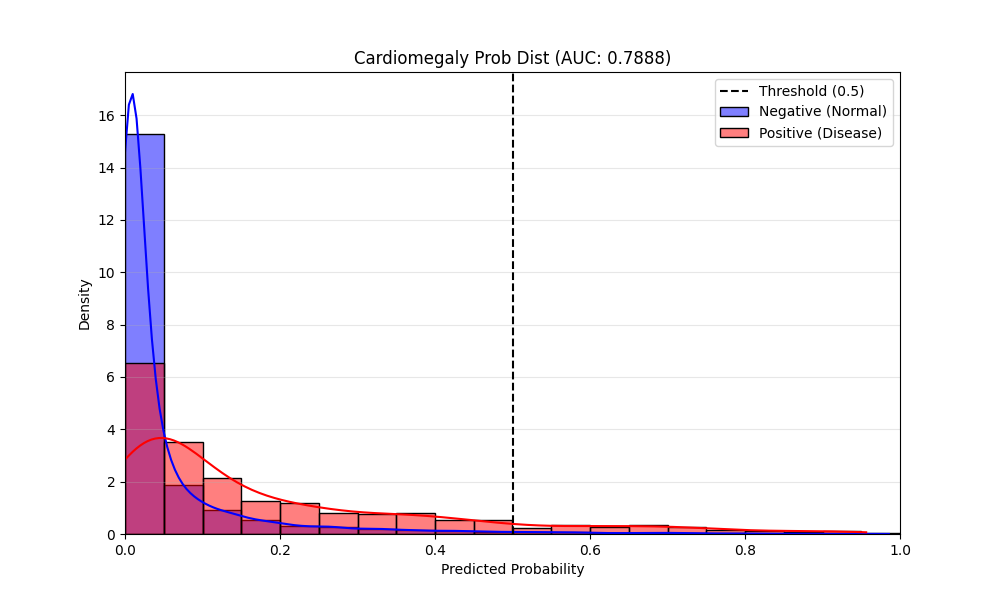
\includegraphics[width=3.0in]{figs/multi_Cardiomegaly.png}
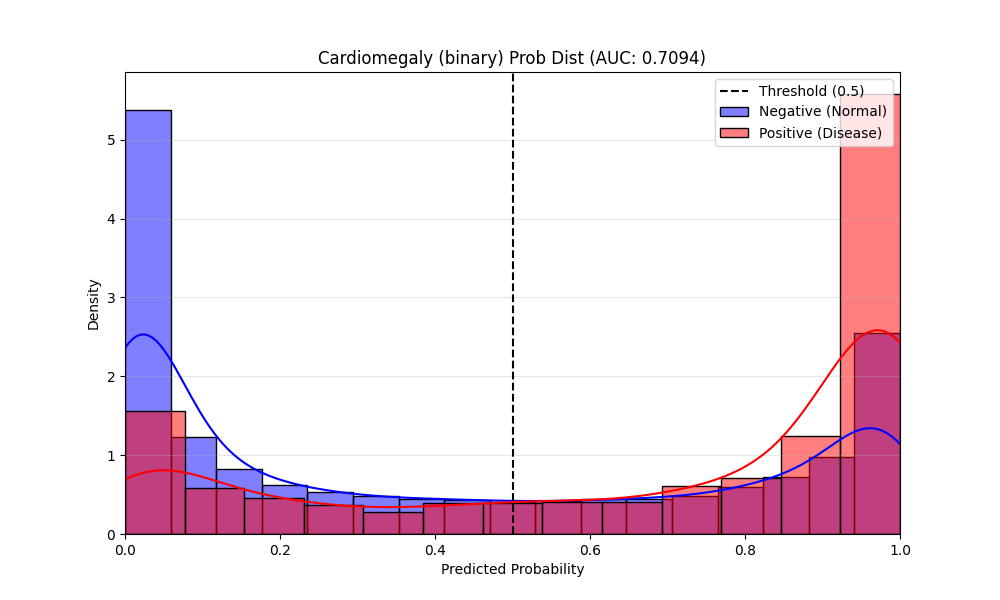
\includegraphics[width=3.0in]{figs/binary_Cardiomegaly.png}
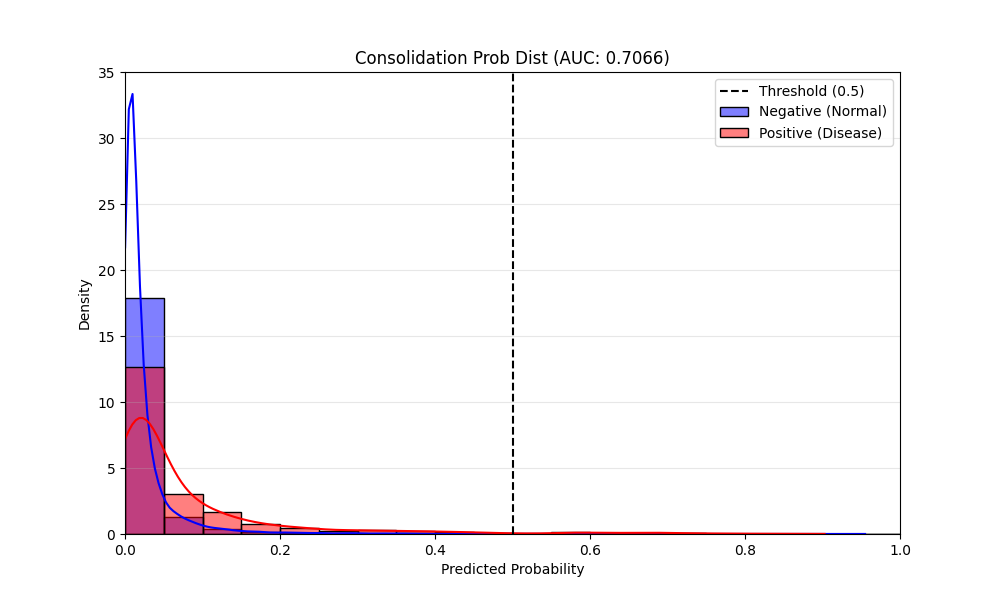
\includegraphics[width=3.0in]{figs/multi_Consolidation.png}
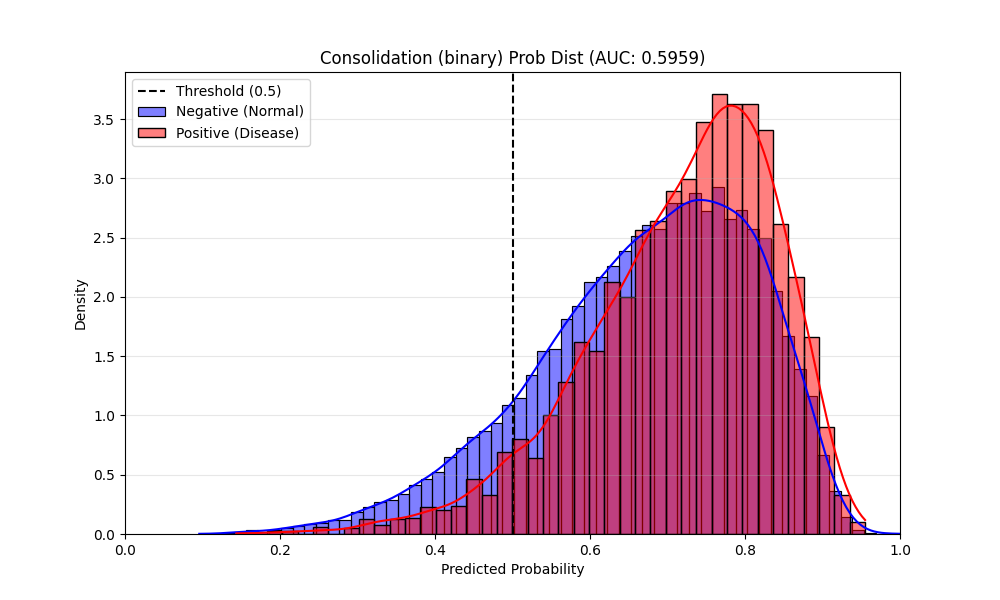
\includegraphics[width=3.0in]{figs/binary_Consolidation.png}
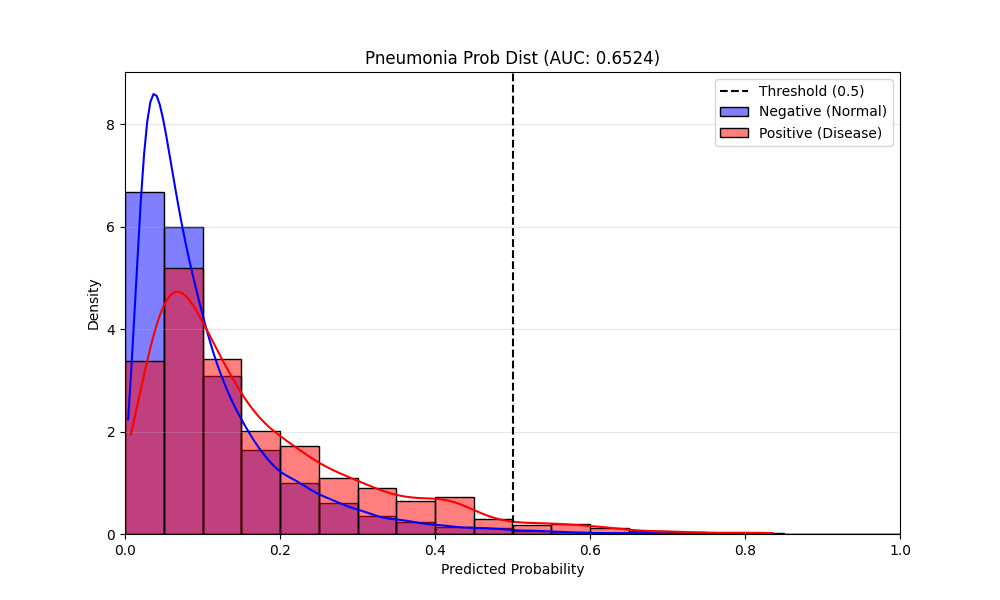
\includegraphics[width=3.0in]{figs/multi_Pneumonia.png}
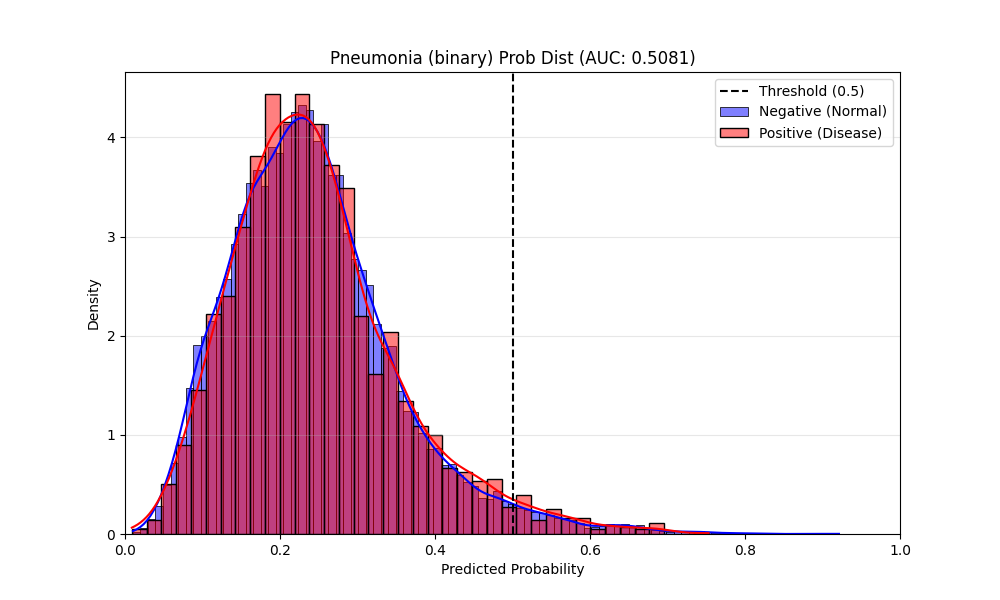
\includegraphics[width=3.0in]{figs/binary_Pneumonia.png}
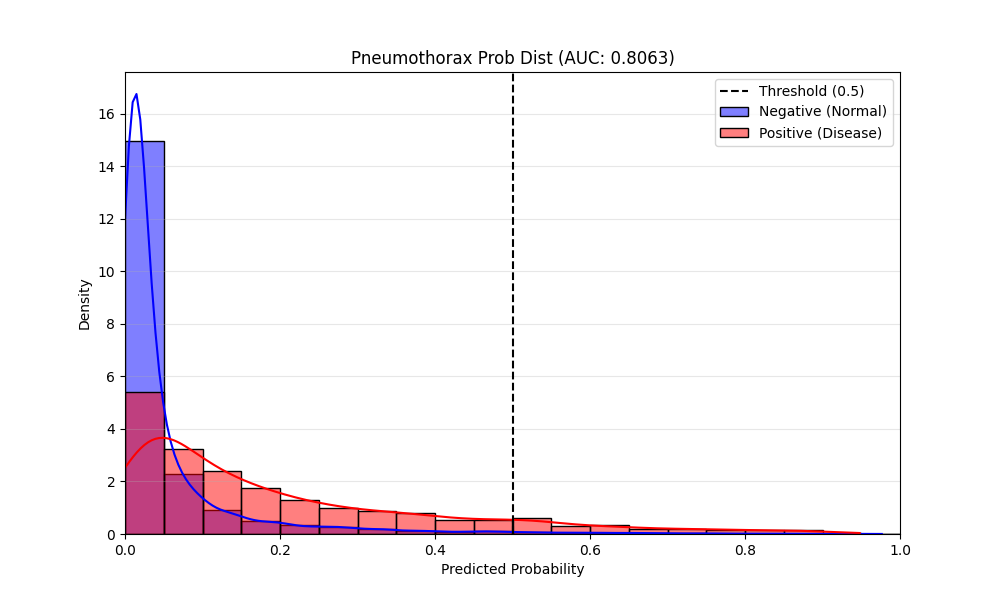
\includegraphics[width=3.0in]{figs/multi_Pneumothorax.png}
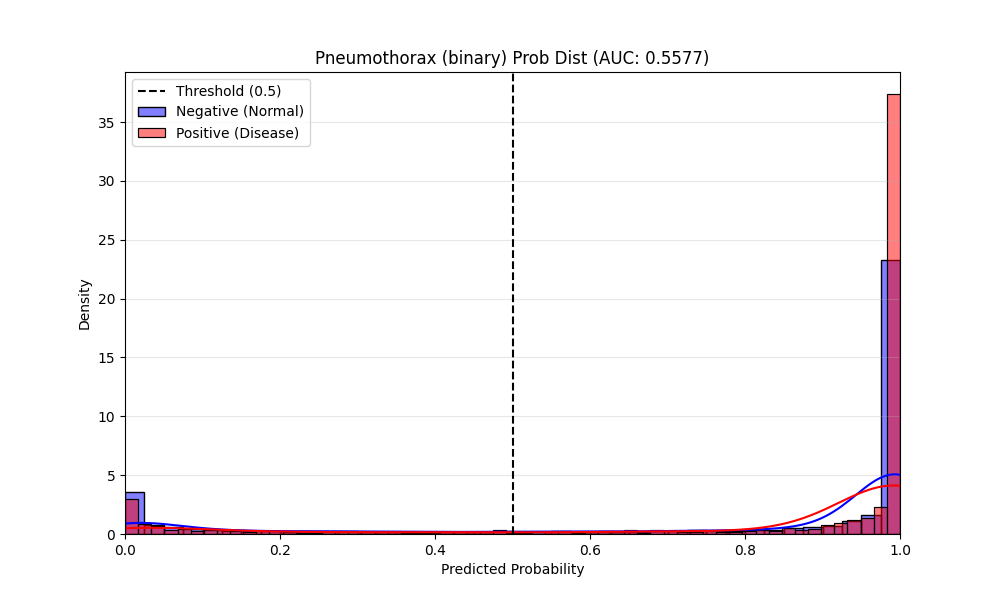
\includegraphics[width=3.0in]{figs/binary_Pneumothorax.png}
\end{center}
\caption{\textcolor{red}{Output probabilities of the trained ICP-L (left column) and the binary classification models (right column).}}
\label{fig:prop}
\end{figure*}

\section{Discussion}
\textcolor{black}{
This work investigates whether class-specific architectural decoupling and saliency-aware optimization can improve both diagnostic performance and saliency-based interpretability. The results suggest that the proposed framework can alleviate insufficient saliency differentiation between true and false classes while maintaining or improving AUC across multiple chest X-ray settings. By replacing the shared final block with Interpretable Class Parallelism (ICP) and optimizing saliency behavior through Functionality Loss and Boost Loss, our method provides a practical route toward more transparent CAD models.}

\textcolor{black}{The variable performance of Stage 2 in certain cases \textcolor{red}{likely} stems from its reliance on the quality of saliency maps generated in Stage 1. \textcolor{red}{Because} Boost Loss depends on masked images derived from Stage 1 saliency maps, suboptimal saliency maps can weaken the regularization signal and may lead to limited interpretability gains. This observation highlights an important practical implication: when explanations are used inside the training loop, explanation quality directly affects downstream optimization.}

\textcolor{black}{\textcolor{red}{The generalizability of our method across diverse clinical settings may be limited by variations in imaging protocols and patient populations.} While the BD metric provides a structured way to quantify interpretability, it depends on accurately defined critical regions and may not capture all clinically meaningful attention patterns. Nonetheless, \textcolor{red}{the improved interpretability enhances transparency, which can foster clinician trust and aid error detection, although} human oversight remains essential in all medical AI applications.}

\textcolor{black}{Future research should \textcolor{red}{develop inherently interpretable architectures that rely less on} multi-stage or auxiliary training procedures. Additionally, there is a need for more comprehensive evaluation metrics that can capture multiple dimensions of interpretability, including clinical relevance, spatial coherence, and user trust. \textcolor{red}{Domain adaptation techniques tailored to the variability of medical images across institutions} will further support model robustness. Addressing these challenges will be essential for advancing computer-aided diagnosis (CAD) systems that are not only accurate but also interpretable, trustworthy, and practically useful in real-world clinical settings.
}


\section{Conclusion}

\textcolor{black}{This work addressed the challenge of improving performance and saliency-based interpretability in multi-label medical image classification. First, we formalized true and false classes at the sample level, providing a framework for analyzing class-wise saliency differentiation. Second, we introduced Interpretable Class Parallelism (ICP), which generates class-specific final representations and improves the differentiation between true- and false-class saliency maps. Third, we proposed Functionality Loss and Detailed-CAM (DCAM) to explicitly optimize saliency behavior during training. Fourth, we introduced a Stage 2 training procedure with Boost Loss, which uses saliency-guided masked inputs to regularize prediction consistency and saliency responses. Finally, we proposed the Bounding-box Difference (BD) metric for quantitatively assessing relative true- and false-class activation inside annotated diagnostic regions.}

\textcolor{black}{Across chest X-ray datasets, the proposed framework improves AUC and saliency-differentiation metrics in many of the evaluated settings, although the improvements are not uniform across all datasets, model widths, and interpretability metrics. These results indicate that class-specific representation learning and saliency-aware regularization are promising directions for developing CAD models that are not only accurate but also easier to inspect through visual evidence. Future work should further evaluate the robustness of this framework under external distribution shifts, broader clinical annotations, and additional medical imaging modalities.}

\bibliographystyle{unsrt}
\bibliography{Reference}

\newpage

\appendix
\addcontentsline{toc}{section}{Appendix}
\section*{Appendix}

% \section{Comparative Analysis of Saliency Maps from CNN and Attention Maps from Transformer in Medical Diagnostics}

% Although Transformer-based models display powerful performances compared to CNNs especially in large datasets, regarding the interpretability, we should carefully analyze both models. In this context, \textit{until now}, the trustworthiness of the saliency maps generated by CNNs can be slightly more advantageous over Transformers, especially in clinical environments for the several reasons. 

% One of the benefits of CNN-based saliency maps is their intuitiveness and interpretability. Saliency maps of CNNs are designed to focus on local features that are critical for diagnosis. This is particularly important in medical imaging, where identifying areas of pathology, such as a tumor or lesion, can directly inform clinical decision-making. In contrast, attention maps from the Transformer models show patch-level relationships capturing global dependencies rather than sharp regions that are critical to the final decision. 

% Furthermore, CNN saliency maps produce more focused and localized explanations that align well with how radiologists and clinicians interpret medical images. In contrast, highly activated patches in Transformer-based attention maps do not have to be critical evidence for the classification results. This makes it challenging for clinicians to interpret the relevance of attention maps in a diagnostic context. Therefore, in cases where precise localization of abnormalities is essential, such as detecting small nodules in a lung X-ray, CNNs offer a distinct advantage.

% Additionally, in CNNs, saliency maps can differ significantly even when class scores are identical, due to the spatial independence and localized feature extraction of convolutional filters. In contrast, Transformers rely on global self-attention mechanisms, where identical class scores often result in similar attention distributions, leading to nearly identical saliency maps. This difference arises from the lack of spatial dependency and the linearity of attention computations in Transformers, making them less sensitive to localized variations. 

\section{Related works}

\textbf{Interpretable AI (XAI).} \textcolor{red}{When deep learning models are applied to real-world data, implausible decision evidence is often a barrier in many fields. In the medical domain, for example, conventional deep learning approaches are criticized for their instability and implausibility \cite{15, 16}. Because a wrong diagnosis can have catastrophic consequences, models with both high explainability and high performance are in demand \cite{12,13,14}. Saliency methods are therefore widely adopted in computer vision \cite{22,23,24,25,26,27,28,29,30}, especially in the medical domain \cite{19,20,21}, for their interpretability.} 

\textcolor{red}{Several methods \cite{5,6,7} improve on pioneering work \cite{4,1,2} to produce better saliency maps. These methods, however, are post-hoc and do not address the training procedure itself. They attribute low-quality saliency maps to the explanation tool.} \textit{\textcolor{red}{Is a low-quality saliency map the result of poor training or of a poor explanation tool?}} \textcolor{red}{We argue that low-quality saliency maps indicate a poor training procedure.} 

\textcolor{red}{To address this problem, one approach \cite{8} disentangles features and feeds them into separate neural networks, but it is limited to multi-layer perceptrons. Like \cite{8}, we aim to improve the training procedure itself, and we do so with} Interpretable Class Parallelism (ICP) \textcolor{red}{rather than by modifying the explanation tools.}

\textcolor{red}{Several metrics exist for saliency methods \cite{9, 17, 18}. However, they cannot evaluate the difference between true- and false-class saliency maps or whether the saliency map covers the most critical region of the input image. We fill this gap by proposing the Bounding-box Difference (BD) metric.}

\textcolor{red}{Moreover, existing saliency tools are designed for multi-class classification \cite{4,1,2,5,6,7,10}. Multi-label classification has more than one correct label, so saliency map generation must be reconsidered for this task.} 

\textbf{Debiased Learning.} \textcolor{red}{Deep learning models often learn shortcuts \cite{31} to improve their performance, because they prefer certain attributes, such as color or texture, to others \cite{32}. This tendency worsens when the dataset itself is biased. For example, if most images of the class bird have sky backgrounds, the model classifies bias-aligned samples, whose background matches this bias, better than bias-conflicting samples, whose background does not \cite{33}. In the medical domain, images of patients with a particular disease may carry specific artifacts such as hospital labels or tags. The model may then decide whether a patient has the disease from these artifacts rather than from the image content that human experts examine. A model should instead decide based on intrinsic attributes rather than peripheral ones. Several works address this problem through debiased learning} \cite{34, 35, 36, 37, 38, 39, 40}.

\section{\textcolor{red}{Implementation Details}}

\label{Appendix2}

\textbf{Hyperparameters.} \textcolor{red}{For all experiments, we used the binary cross-entropy (BCE) loss without a learning rate scheduler. To measure BD and deletion scores, we used Grad-CAM for its sharp localization. For the NIH CXR 14 and CheXpert experiments, we used the following settings. We resized the original images to $150 \times 150$ pixels and applied no augmentation other than normalization. We used the SGD optimizer \cite{50} with momentum 0.9 and weight decay 0.0001, a learning rate of 0.01, 20 epochs, and a batch size of 32. For ICP-T on NIH CXR 14, we scaled the Functionality Loss by 0.1. We chose ResNet18 \cite{49} as the base architecture of ICP for its computational and memory efficiency, and we used 1, 128, 256, and 512 channels in its last parallel convolutional blocks, which we call ICP-T, ICP-M, ICP-L, and ICP-XL, respectively. Figure \ref{fig:ICP} shows this architecture.}

\textbf{Metrics.} \textcolor{red}{We evaluated models with AUC, BD, and deletion scores. AUC, the area under the receiver operating characteristic curve, measures performance, and BD and deletion scores measure interpretability. DT is the AUC on the original, unmodified input minus the AUC on the image from which the highly activated regions of the true-class saliency map are erased. DF is computed in the same way with the false-class saliency map. A high DT score therefore means that the model activated the critical region that strongly affects AUC, and a low DF score means that the model did not mistake critical regions for evidence of false classes. We used a threshold of 0.7: to compute deletion scores, we erased pixels with saliency above 0.7 and fed the resulting image into the model.}



\section{Additional experimental results}

\subsection{MIMIC dataset}

To further evaluate the proposed Interpretable Class Parallelism (ICP), we conducted experiments \textcolor{red}{on MIMIC-CXR, a large-scale chest X-ray dataset commonly used in clinical research. This dataset allows us to test the robustness and scalability of ICP in a realistic clinical setting. We trained the model with the same architecture and procedure as in the previous experiments and focused on whether Functionality Loss and Boost Loss improve performance and interpretability.}

\textcolor{black}{In the Stage 1 experiments in Table \ref{mimic1}, the ICP-M model with Functionality Loss achieved an AUC of 75.04, showing a noticeable improvement over the evaluated baseline models. Regarding interpretability, several ICP \textcolor{red}{variants} also achieved improved DT-DF (the difference between DT and DF). These results suggest that ICP and Functionality Loss can improve both classification performance and saliency differentiation on MIMIC-CXR, although the magnitude of improvement depends on the ICP width and loss configuration.}

\textcolor{red}{In Stage 2, however, our method achieved higher or similar AUC with ICP-T, ICP-M, and ICP-L but did not improve the interpretability scores. This result shows that Stage 2 does not yet generalize stably across datasets, even though it improved performance on other datasets such as NIH CXR 14.}

\begin{table*}
    \centering
    {\resizebox{\textwidth}{!}{
    \begin{tabular}{c|cc|c|ccc|c}
        \toprule
        \multicolumn{8}{c}{\textbf{MIMIC-CXR}}\\
        \midrule
        \textbf{Method} & $\mathbf{\mathcal{L}_{AS}}$ & $\mathbf{\mathcal{L}_{func}}$& \textbf{\textcolor{magenta}{AUC $\uparrow$}} & \textbf{\textcolor{cyan}{DT $\uparrow$}}& \textbf{\textcolor{cyan}{DF $\downarrow$}}& \textbf{\textcolor{cyan}{DT - DF $\uparrow$}} & \textbf{\# Params}\\
        \midrule
        \rowcolor{Gray}
        DenseNet121 & X & X & 74.02 $(\pm0.24)$ & 2.42 $(\pm0.76)$ & 1.75 $(\pm0.90)$& 0.42 $(\pm0.49)$ & 7M\\
        \rowcolor{Gray}
        EfficientNetB7 & X & X & 74.24 $(\pm0.12)$& 6.51 $(\pm0.85)$ & 2.38 $(\pm0.80)$& 4.10 $(\pm1.05)$ & 63M\\
        \rowcolor{Gray}
        ConvNeXtBase & X & X & 70.56 $(\pm0.09)$ & 1.44 $(\pm0.25)$ & 0.75 $(\pm0.18)$& 0.71 $(\pm0.10)$& 87M\\
        \rowcolor{Gray}
        ViT & X & X & 71.30 $(\pm0.56)$ & \textbf{14.98} $\bm{(\pm1.11)}$ & 14.98 $(\pm1.11)$ & 0.00 $(\pm0.00)$ &  85M\\
        \rowcolor{Gray}
        ResNet18 & X & X & 70.47 $(\pm0.14)$ & 8.88 $(\pm0.26)$ & 7.77 $(\pm0.71)$ & 1.04 $(\pm0.87)$ & 11M\\
        \rowcolor{Gray}
        ResNet18 & O & X & 70.98 $(\pm1.11)$ & 6.93 $(\pm0.55)$ & 8.51 $(\pm0.61)$ & -1.12 $(\pm1.12)$ & 11M\\
        \midrule
        ResNet18 & X & O & 71.18 $(\pm0.61)$ & 8.85 $(\pm1.01)$ & 7.72 $(\pm0.31)$ & 1.12 $(\pm0.70)$ & 11M\\
        ResNet18 & O & O & 70.97 $(\pm0.25)$ & 7.49 $(\pm1.63)$ & 7.61 $(\pm0.48)$ & -0.12 $(\pm2.11)$ & 11M\\
        \midrule
        ICP-T & X & X & 72.30 $(\pm0.19)$ & 0.69 $(\pm0.09)$ & 0.00 $(\pm0.01)$ & 0.67 $(\pm0.09)$ & 11M\\
        ICP-T & O & X & 72.55 $(\pm0.40)$ & 0.73 $(\pm0.15)$ & 0.00 $(\pm0.03)$ & 0.73 $(\pm0.19)$ & 11M\\
        ICP-T & X & O & 72.35 $(\pm0.09)$ & 1.49 $(\pm1.13)$ & 0.02 $(\pm0.04)$ & 1.44 $(\pm1.11)$ & 11M\\
        ICP-T & O & O & 72.09 $(\pm0.02)$ & 2.50 $(\pm0.37)$ & 0.00 $(\pm0.06)$ & 2.54 $(\pm0.34)$ & 11M\\
        \midrule
        ICP-M & X & X & 73.35 $(\pm0.67)$ & 2.98 $(\pm1.52)$ & 0.00 $(\pm0.00)$ & 2.98 $(\pm1.52)$ & 21M\\
        ICP-M & O & X & 73.34 $(\pm0.16)$ & 0.45 $(\pm0.16)$ & 0.00 $(\pm0.00)$ & 0.45 $(\pm0.16)$ & 21M\\
        \rowcolor{LemonChiffon1}
        ICP-M & X & O & \textbf{75.04} $\bm{(\pm0.57)}$ & 11.01 $(\pm1.35)$ & 0.00 $(\pm0.00)$ & 11.01 $(\pm1.35)$ & 21M\\
        ICP-M & O & O & 73.59 $(\pm0.68)$ & 1.16 $(\pm0.05)$ & -0.01 $(\pm0.01)$ & 1.17 $(\pm0.06)$ & 21M\\
        \midrule
        ICP-L & X & X & 73.05 $(\pm0.89)$ & 2.46 $(\pm0.98)$ & 0.00 $(\pm0.00)$ & 2.46 $(\pm0.98)$ & 45M\\
        ICP-L & O & X & 73.93 $(\pm0.21)$ & 0.71 $(\pm0.41)$ & 0.00 $(\pm0.01)$ & 0.72 $(\pm0.42)$ & 45M\\
        ICP-L & X & O & 74.97 $(\pm0.80)$ & 11.27 $(\pm0.89)$ & -0.21 $(\pm0.21)$ & 11.49 $(\pm1.11)$ & 45M\\
        ICP-L & O & O & 73.88 $(\pm0.83)$ & 5.18 $(\pm4.58)$ & -0.04 $(\pm0.04)$ & 5.21 $(\pm4.61)$ & 45M\\
        \midrule
        ICP-XL & X & X & 73.68 $(\pm0.12)$ & 0.99 $(\pm0.72)$ & 0.00 $(\pm0.01)$ & 1.00 $(\pm0.72)$ & 128M\\
        ICP-XL & O & X & 72.50 $(\pm1.20)$ & 0.46 $(\pm0.02)$ & 0.00 $(\pm0.00)$ & 0.45 $(\pm0.02)$ & 128M\\
        ICP-XL & X & O& 74.62 $(\pm1.00)$ & 11.90 $(\pm1.06)$ & \textbf{-0.33} $\bm{(\pm0.10)}$ & \textbf{12.53} $\bm{(\pm1.15)}$ & 128M\\
        ICP-XL & O & O & 73.47 $(\pm0.25)$ & 0.48 $(\pm0.20)$ & 0.00 $(\pm0.01)$ & 0.48 $(\pm0.18)$ & 128M\\
        \bottomrule
    \end{tabular}
    }}
    \caption{\textcolor{red}{Results on MIMIC-CXR with 20 training epochs. Gray rows are baselines without our methods, and white rows are variants of our methods.}}
    \label{mimic1}
\end{table*}

\begin{table*}
    \centering {
    \begin{tabular}{c|c|c|ccc}
        \toprule
        \multicolumn{6}{c}{\textbf{MIMIC-CXR}}\\
        \midrule
        \textbf{Method} & \textbf{Stage 2} & \textbf{\textcolor{magenta}{AUC $\uparrow$}} & \textbf{\textcolor{cyan}{DT $\uparrow$}}& \textbf{\textcolor{cyan}{DF $\downarrow$}}& \textbf{\textcolor{cyan}{DT - DF $\uparrow$}}\\
        \midrule
        \rowcolor{Gray}
        ICP-T & X & 74.71 & 5.54 & 0.00 & 5.54 \\
        ICP-T & O & 74.98 & 4.29 & 0.00 & 4.29 \\
        \midrule
        \rowcolor{Gray}
        ICP-M & X & 77.19 & 7.81 & 0.00 & 7.81 \\
        ICP-M & O & 77.11 & 6.38 & 0.00 & 6.38 \\
        \midrule
        \rowcolor{Gray}
        ICP-L & X & 71.44 & 13.35 & -0.01 & 13.36 \\
        ICP-L & O & 77.01 & 4.80 & 0.00 & 4.80 \\
        \midrule
        \rowcolor{Gray}
        ICP-XL & X & 77.22 & 13.66 & -0.89 & 14.56 \\
        ICP-XL & O & 75.98 & 1.82 & 0.00 & 1.82 \\
        \bottomrule
    \end{tabular}}
    \caption{\textcolor{red}{Results on MIMIC-CXR with 40 training epochs. We compare models with and without a data augmentation strategy. $\tau$ is the masking threshold, set to 0.6, and the remaining pixels are multiplied by 0.4.}}
    \label{mimic2}
\end{table*}





% \subsection{The Comparison of the Number of Model Parameters}

% To analyze the efficiency of our proposed methodology, we compared the number of parameters in various models. As shown in Table \ref{tab:1} and Table \ref{tab:2}, the ICP models were implemented with varying channel sizes, specifically ICP-T, ICP-M, ICP-L, and ICP-XL. Their last parallel blocks are composed of 1, 128, 256, 512 channels. While the ICP-XL model generally exhibited superior performances and interpretability, the ICP-M and ICP-L models also delivered competitive results. This comparison highlights that although ICP-XL often achieves the best results, ICP-M and ICP-L offer a good balance between performance and computational efficiency, making them viable options in resource-constrained environments.

\begin{figure*}
\begin{center}
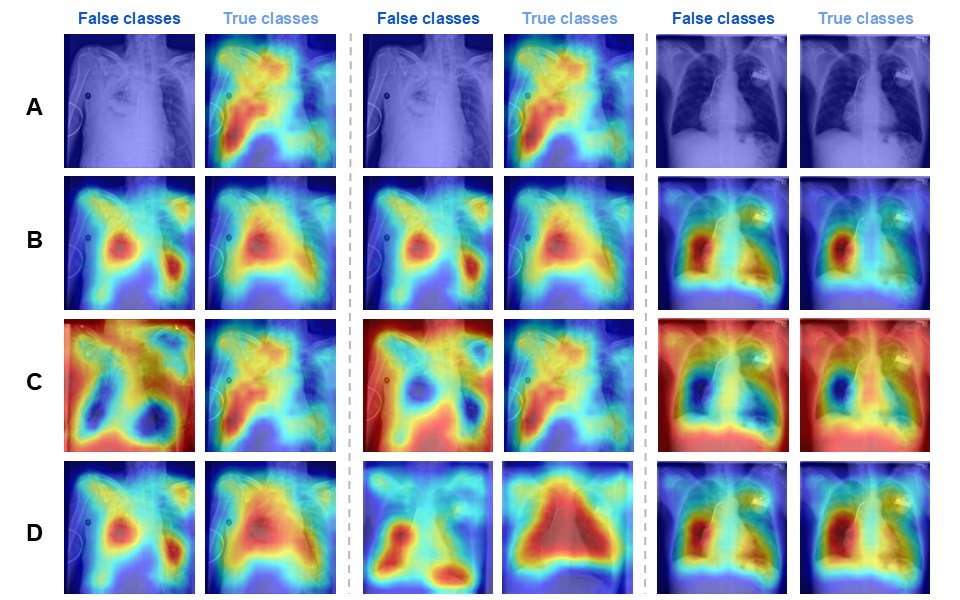
\includegraphics[width=5in, height=3.2in]{Figure2.png}
\caption{\textcolor{red}{Comparison of saliency maps from Grad-CAM and its modifications. The saliency maps for true and false classes were generated with each version of Grad-CAM on ICP-M.}}
\label{fig:CAM}
\end{center}
\end{figure*}



\subsection{Verification of DCAM}

\textcolor{red}{We use DCAM to improve the interpretability of the model's decision-making. DCAM represents activation values over their full range rather than focusing on localization. Using it in the Functionality Loss effectively suppresses false-class saliency maps. Table \ref{tab:5} summarizes the quantitative evaluation of DCAM. With ICP-M, ICP-L, and ICP-XL, models with DCAM outperform those without it in both interpretability and performance. Figure \ref{fig:CAM} shows the saliency maps produced by each modification. Equations \ref{eq:14}--\ref{eq:17} give the formulations used to obtain rows A to D, and Section \ref{sec:Methods} defines their variables.}

\begin{equation}
\label{eq:14}
            \frac{1}{Z}\sum_{i}\sum_{j}\frac{\partial y_c}{\partial A^{k}_{ij}}, 
            \text{ReLU}\bigg(\sum_{k}\alpha_{k,\text{CAM}} * A^{k}\bigg)
\end{equation}

\begin{equation}
\label{eq:15}
            \sigma\bigg(\frac{1}{Z}\sum_{i}\sum_{j}\frac{\partial y_c}{\partial A^{k}_{ij}}\bigg), 
            \text{ReLU}\bigg(\sum_{k}\alpha_{k,\text{CAM}} * A^{k}\bigg)
\end{equation}

\begin{equation}
\label{eq:16}
            \frac{1}{Z}\sum_{i}\sum_{j}\frac{\partial y_c}{\partial A^{k}_{ij}}, 
            \sigma\bigg(\sum_{k}\alpha_{k,\text{CAM}} * A^{k}\bigg)
\end{equation}

\begin{equation}
\label{eq:17}
            \sigma\bigg(\frac{1}{Z}\sum_{i}\sum_{j}\frac{\partial y_c}{\partial A^{k}_{ij}}\bigg), 
            \sigma\bigg(\sum_{k}\alpha_{k,\text{CAM}} * A^{k}\bigg)
\end{equation}

\textcolor{red}{Because Grad-CAM erases negative values, the false-class saliency maps have no activation. Their sum is then already near zero, so the Functionality Loss becomes zero, which is problematic. The third row is also problematic because it highlights peripheral regions at random rather than critical regions. The second and last rows suit the Functionality Loss, because they activate the false-class saliency maps and highlight critical regions. Empirically, the last row (DCAM) gives the best results.} 

\begin{table*}
    \centering
    \resizebox{\textwidth}{!}{\begin{tabular}{cc|c|cccc}
        \toprule
        \multicolumn{7}{c}{\textbf{NIH CXR 14}}\\
        \midrule
        \textbf{Method} & \textbf{CAM} & \textbf{\textcolor{magenta}{AUC $\uparrow$}} & \textbf{\textcolor{cyan}{BD $\uparrow$}} & \textbf{\textcolor{cyan}{DT $\uparrow$}}& \textbf{\textcolor{cyan}{DF $\downarrow$}}& \textbf{\textcolor{cyan}{DT - DF $\uparrow$}}\\
        \midrule
        \rowcolor{Gray}
        ResNet18 & GradCAM & 72.63 $(\pm0.65)$& 2.86 $(\pm0.47)$& 1.41 $(\pm0.45)$& 0.00 $(\pm0.00)$& 1.41 $(\pm0.45)$\\
        \rowcolor{Gray}
        ICP-T & GradCAM & 69.13 $(\pm0.57)$& 3.38 $(\pm2.80)$& 0.21 $(\pm0.17)$& 0.01 $(\pm0.01)$ & 0.21 $(\pm0.17)$\\
        \rowcolor{Gray}
        ICP-M & GradCAM& 71.94 $(\pm0.67)$& 8.95 $(\pm4.82)$& 3.32 $(\pm0.73)$ & 0.00 $(\pm0.00)$& 3.32 $(\pm0.73)$\\
        \rowcolor{Gray}
        ICP-L & GradCAM& 71.46 $(\pm0.16)$& 4.52 $(\pm0.29)$& 3.98 $(\pm1.15)$& 0.00 $(\pm0.00)$& 3.98 $(\pm1.15)$\\
        \rowcolor{Gray}
        ICP-XL & GradCAM& 72.08 $(\pm1.30)$ & 2.21 $(\pm1.70)$ & 2.06 $(\pm1.66)$& 0.00 $(\pm0.00)$ & 2.06 $(\pm1.66)$\\
        \midrule
         ResNet18 & DCAM& 66.97 $(\pm0.25)$ & 2.03 $(\pm 0.45)$& 8.25 $(\pm0.14)$& 6.63 $(\pm0.76)$& 1.62 $(\pm0.62)$\\
        ICP-T & DCAM& 69.55 $(\pm0.86)$ & 8.69 $(\pm6.79)$ & 1.57 $(\pm1.24)$& 0.00 $(\pm0.00)$& 1.56 $(\pm1.24)$\\
        ICP-M & DCAM& 74.38 $(\pm0.88)$ & 16.59 $(\pm1.52)$ & 5.75 $(\pm0.45)$& 0.00 $(\pm0.00)$& 5.75 $(\pm0.45)$\\
        ICP-L & DCAM& 74.38 $(\pm0.16)$ & 16.10 $(\pm1.22)$ & 5.46  $(\pm0.70)$& 0.03 $(\pm0.02)$& 5.43 $(\pm0.72)$\\
        ICP-XL & DCAM& \textbf{74.64 $\bm{(\pm0.76)}$} & \textbf{17.88 $\bm{(\pm1.69)}$} & \textbf{6.84} $\bm{(\pm0.39)}$& \textbf{0.02 $\bm{(\pm0.02)}$} & \textbf{6.83 $\bm{(\pm0.37)}$}\\
        \bottomrule
    \end{tabular}}
    \caption{\textcolor{red}{Results of our method when Grad-CAM, instead of DCAM, is used to compute the Functionality Loss.}}
    \label{tab:5}
\end{table*}

\section{Theoretical guarantee}
\label{Appendix:D}

\textcolor{red}{Our methods aim to make the saliency maps of true and false classes more independent, thereby preventing shortcut learning. Making saliency maps independent corresponds directly to reducing their inner product.} 

\textcolor{red}{Let} $X$ \textcolor{red}{be} the input image and $\mathcal{S}_i = P_i(X)$ \textcolor{red}{the} saliency map for class $i$\textcolor{red}{, and let} $\hat{\mathcal{S}}_i = \frac{\mathcal{S}_i}{||\mathcal{S}_i||}$ \textcolor{red}{be the normalized saliency map. The objective of our two methods can then be written as:}

\begin{equation*}
 Score = \frac{\sum_{i \in True} \mathcal{S}_{i}}{\sum_{i \in True} \sum_{j \in False} <\hat{\mathcal{S}}_i, \hat{\mathcal{S}}_j> + \sum_{j \in False}\mathcal{S}_{j} + \epsilon}    
\end{equation*}

\textcolor{black}{$<\cdot>$ \textcolor{red}{denotes the} inner product, and $i$ and $j$ \textcolor{red}{index the true and false classes, respectively. Maximizing this score requires increasing the intensity values of true classes and decreasing those of false classes. As a result, the \textit{Score} is proportional to the gap between them.}}

\begin{equation*}
    Score \propto \sum_{i \in True} \mathcal{S}_i - \sum_{j \in False} \mathcal{S}_j
\end{equation*}

\textcolor{red}{In} Grad-CAM, the sum of saliency map values is proportional to the class score. 

\begin{equation*}
    y_c = \sum_{y = 1}^H \sum_{x = 1}^W \mathcal{S}^{yx}
\end{equation*}

$y_c$ is the \textcolor{red}{score of class $c$, $x$ and $y$ are pixel indices, and $H$ and $W$ are the height and width of the image. Hence, increasing the gap between the summed saliency of true and false classes also increases the gap between their class scores.}

\begin{equation*}
    Score \propto \sum_{i \in True} \mathcal{S}_i - \sum_{j \in False} \mathcal{S}_j \propto \sum_{i \in True} y_i - \sum_{j \in False} y_j
\end{equation*}

As a result, maximizing $Score$ \textcolor{red}{increases $\sum_{i \in True} y_i$} and decreases \textcolor{red}{$\sum_{j \in False} y_j$, which explains how} the combination of ICP and Functionality Loss \textcolor{red}{can improve} overall diagnostic performance.

\begin{figure*}
\begin{center}
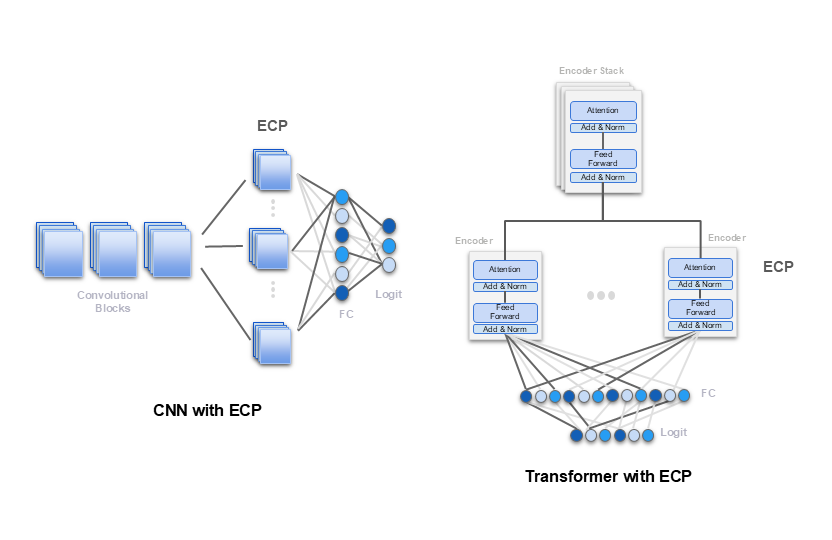
\includegraphics[width=5.5in, height=3.7in]{Figure3.png}
\caption{\textcolor{red}{Structure of ICP. We replicate the last convolutional block once per class, and Functionality Loss assigns each block to its class.}}
\label{fig:ICP}
\end{center}
\end{figure*}

\subsection{\textcolor{red}{Use of Large Language Models in Manuscript Preparation}}
\textcolor{black}{We \textcolor{red}{used} Google\textcolor{red}{'}s Gemini and OpenAI's ChatGPT for language editing and \textcolor{red}{to improve the clarity and scientific quality of the manuscript. The} authors \textcolor{red}{reviewed} all AI-generated suggestions and remain solely responsible for the final scientific content and conclusions.}

\end{document}
